%!TEX root = ../thesis.tex

% *****************************************************************************
% ********************************** CHAPTER 4 ********************************
% *****************************************************************************

\chapter{Implementation}

In the context of distributed systems, middleware for pub/sub communication
plays a fundamental role, as discussed in the previous chapter. This thesis
starts with the idea that embedded systems, particularly those with
heterogeneous processors, can be perceived as a form of distributed system.

While substantial progress has been made in the domain of pub/sub platforms for
traditional distributed systems, the adaptation of such platforms to satisfy
the needs of embedded systems is relatively unexplored territory.
This presents an oppotune starting point leveraging existing knowledge while
navigating the unique challenges inherent in embedded systems.

As seen in the initial chapters, embedded systems have different requisites
from traditional systems.
Solutions in this domain must take into consideratio low latency requirements,
safety considerations, and other specific needs for the specific application.

The primary goal of this project is to realize a pub/sub platform that exploits
the advantages offered by pub/sub communication while satisfying the needs of
embedded systems.

In this chapter are illustrated in detail the implementation of the pub/sub
platform created illustrating the architectural choices.

\section{Architecture}

The proposed pub/sub middleware starts with a layer architecture, carefully
structured to address the unique challenges posed by embedded systems. This
section illustrates the key components residin in each layer, providing
information about their roles, interactions, and contributions to the overall
efficacy of the communication framework.

\begin{figure}[H]
    \centering
    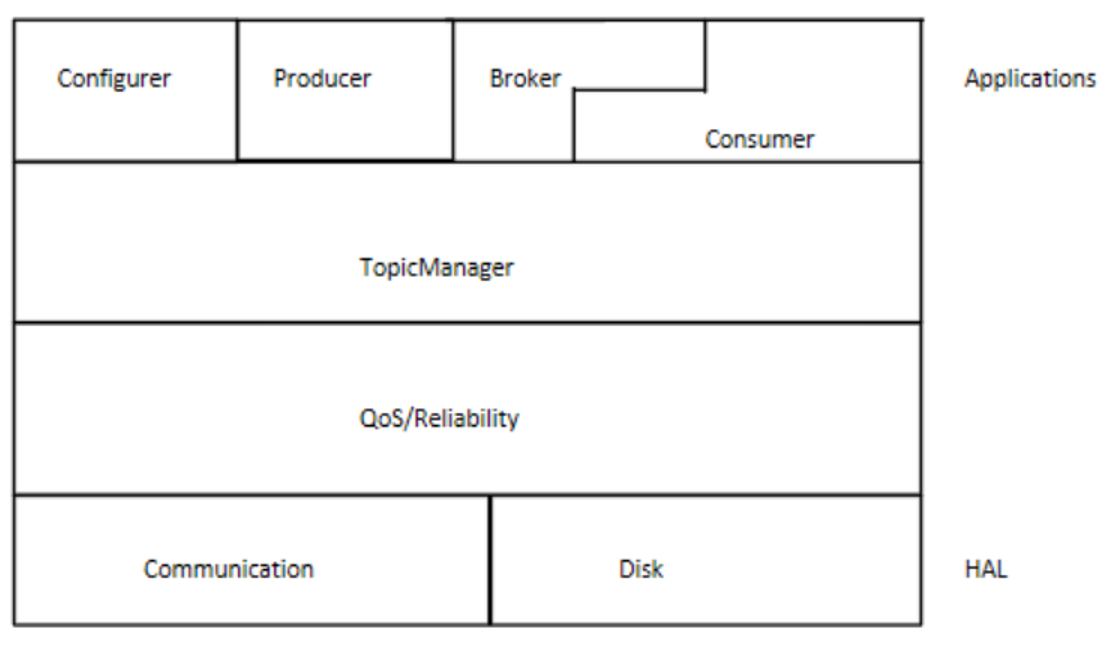
\includegraphics[width=1.0\textwidth]{Figures/architecture_layers.png}
    \caption{Layered architecture of the solution}
\end{figure}

At the top of the architecture resides the Application layer, the interface
through which end-users and system components interact with the pub/sub
middleware. The Application layer provides a user-friendly inteface for
configuring, consuming and producing messages within the ecosystem.
This layer is further subdivided into essential elements:

\begin{itemize}
    \item   Configurer: Responsible for configuring and maintain the
            information about the other components of the system.
    \item   Consumer: Facilitates the consumption of messages and the
            interactions needed for retreiving messages.
    \item   Broker: Serves as intermediary between producers and consumers,
            efficiently routing messages based on established topic
            subscription.
    \item   Producer: initiates the generation of messages into the
            communication network.
\end{itemize}

Under the Application layer, the Topic Manager layer serves as the manager of
all topic-related operations. The layer manages the creation, deletion and
tracks topics within the system. The seamsless coordination of topics is one
of the most important element, making the Topic Manager one of the most
important element to provide flexible and dynamic communication infrastructure.

Coming down from the most abstract layers, the Quality of Service (QoS) layer
introduces elements designed to enhance the middleware's reliability and
safety. Within this layer, mechanisms for topic replication and the possibility
to define custom logic for the distribution of messages between a group of
consumers can be found.

Situated at the bottom of the stack there are the communication and disk
components, which is defined as the Operating System (OS) layer.
The Disk layer introduces a component for persistent data storage; classes
dedicated to saving records on disk have great importance to ensure data
durability.
This layer is particularly important when records have to be preserved beyond
runtime.

The other component at the base of the architecture is the Communication layer.
It plays a fundamental role for facilitating interaction among distributed
components within embedded systems.
Leveraging the APIs provided by Texas Instruments, this layer ensures robust
and efficient communication between diffeerent processors.

\section{Class interactions}

The image (figure \ref{fig:class_diagram}) details the different components
that enable the exchange of messages between producers and consumers in a
distributed environment.

The architecture is composed of vrious entities, including a cluster,
consumer groups, brokers, replicas, partitions, records, prodcuers and
consumers. 

\begin{figure}[H]
    \centering
    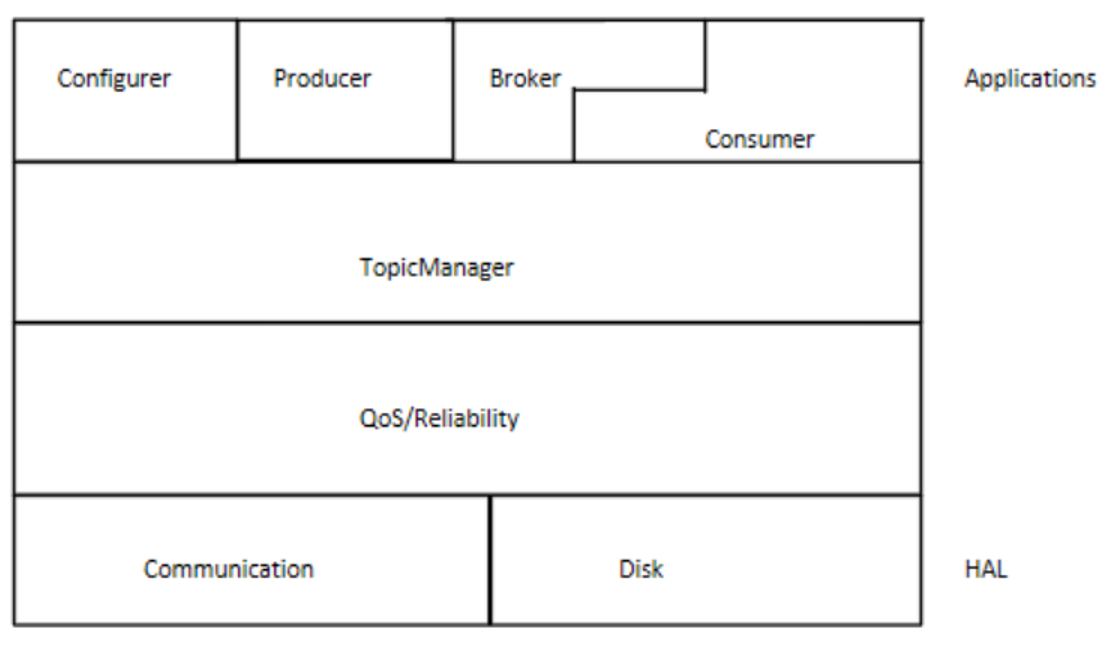
\includegraphics[width=1.0\textwidth]{Figures/architecture_layers.png}
    \caption{Layered architecture of the solution}
    \label{fig:class_diagram}
\end{figure}

The most interesting components are the following ones:

\begin{itemize}
    \item   Cluster: the cluster is the foundation of the middleware, acting as
            a collection of brokers that facilitate message exchange and
            compose the general system.
    \item   Consumer groups: Consumer groups organize consumers into logical
            units, allowing them to divide and conquer the workload of
            consuming messages from a topic. The approach enhances parallelism
            and scalability.
    \item   Replicas: replicas are copies of partitions stored on different
            brokers, providing redundancy and fault tolerance. If the primary
            broker of a partition fails, a replica can take over its role,
            ensuring uninterrupted message delivery.
\end{itemize}

These ideas are taken from Apache kafka and applied to the embedded system
domain.

\section{Class Diagrams}

In the current section the class diagrams for the different layers will be
analyzed.

\subsection{Topic Manager}

The Topic Manager layer is responsible for managing the topic metadata and
handling interactions between producers, consumers and brokers. It is a crucial
component of the middleware, ensuring efficient message exchange and ensuring
the integrity of the messaging system.

\begin{figure}[H]
    \centering
    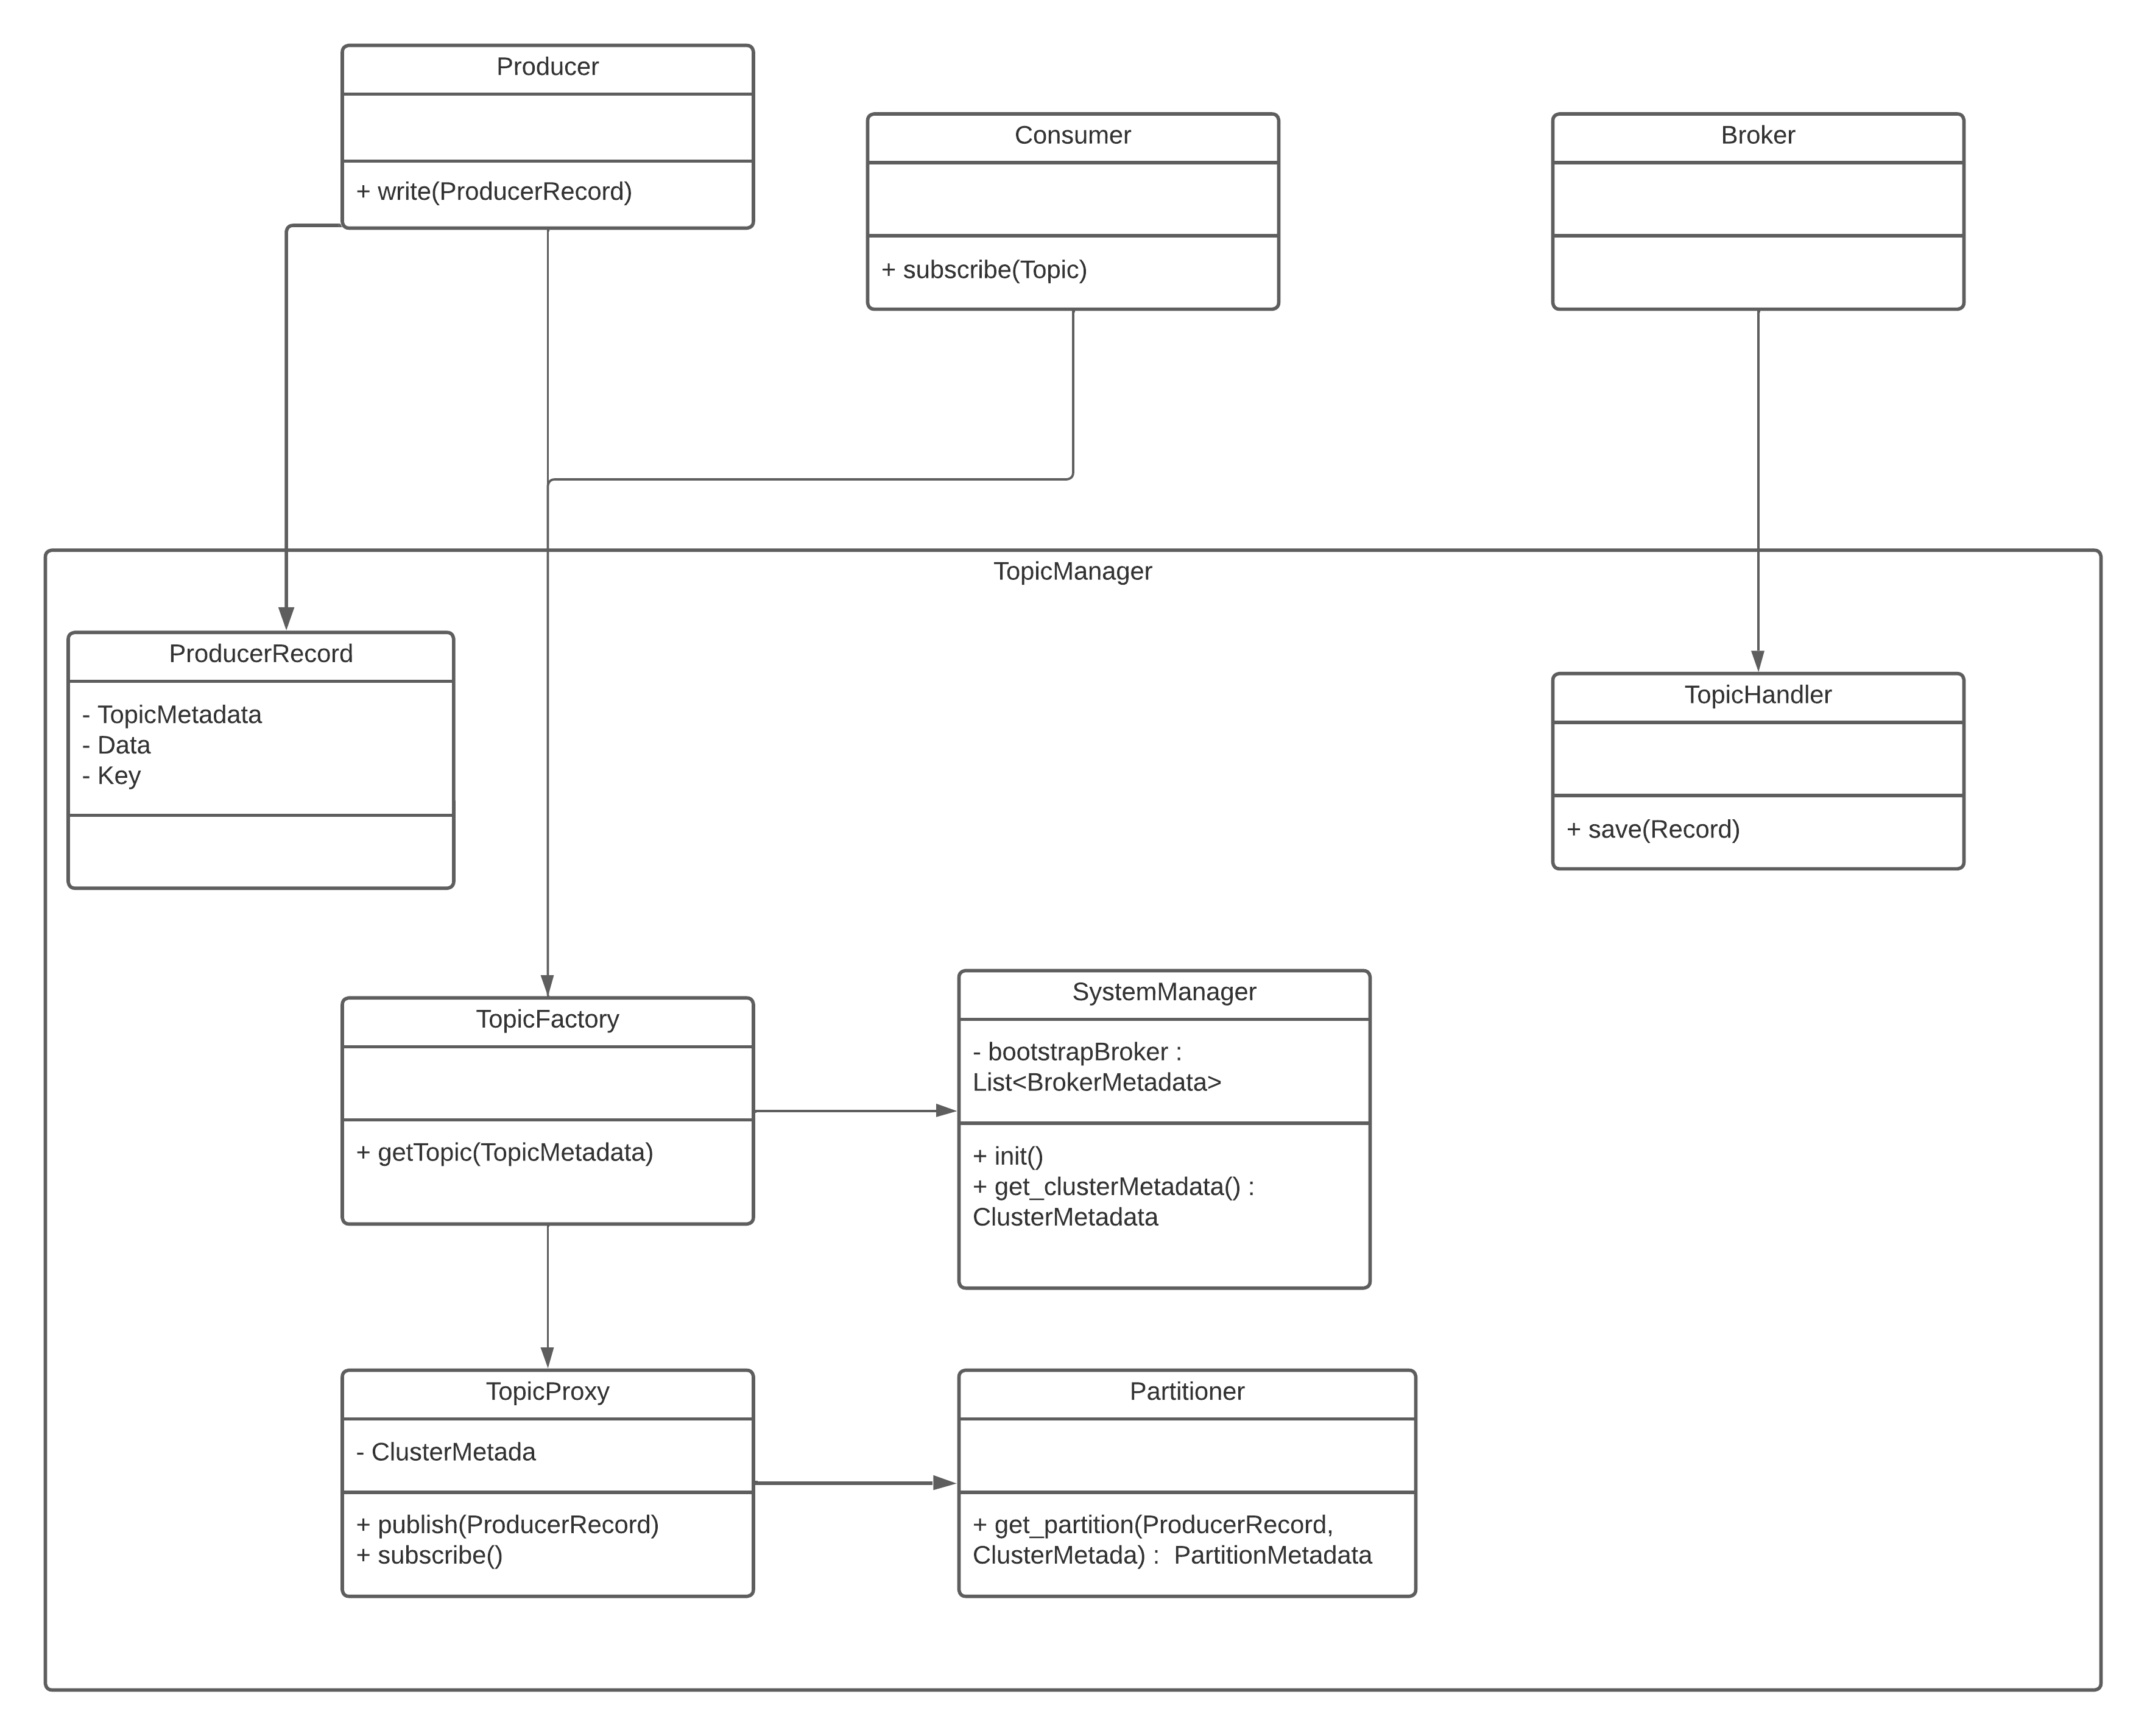
\includegraphics[width=1.0\textwidth]{Figures/class_diagram_topic_manager.png}
    \caption{Class diagram of the topic manager layer}
    \label{fig:class_diagram_topic_manager}
\end{figure}

The topic manager layer interacts with the broker component to maintain the
state of topics, including the creation, deletetion and modification.
It also manages subscriptions, ensuring that consumers are notified of messages
published to topics they are subscribed to. Additionaly, the topic manager
layer handles message routing, directing messages to the appropriate partitions
within each topic.

The topic manager layer is implemented as a collection of components that work
together to provide the necessary functionality. These components include:

\begin{enumerate}
    \item   TopicFactory: this component is responsible for creating new
            topics and managing their metadata. It ensures that topics are
            created with the appropriate configurations and that they are
            registered with the broker.
    \item   TopicHandler: This component handles interactions between producers
            and consumers. It receives messages from producers, adds them to
            the appropriate partitions, and updates topic metadata. It also
            receives subscription requests from consumers and manages
            subscriptions accordingly.
    \item   SystemManager: this component is of fundamental importance for all
            the system operations. It provides a centralized interface for
            managing the communication with the configurer. It also provides
            all the information about the current status of the cluster.
\end{enumerate}

\subsection{QoS}

The QoS layer is responsible for managing the quality of services (QoS) of the
system.

\begin{figure}[H]
    \centering
    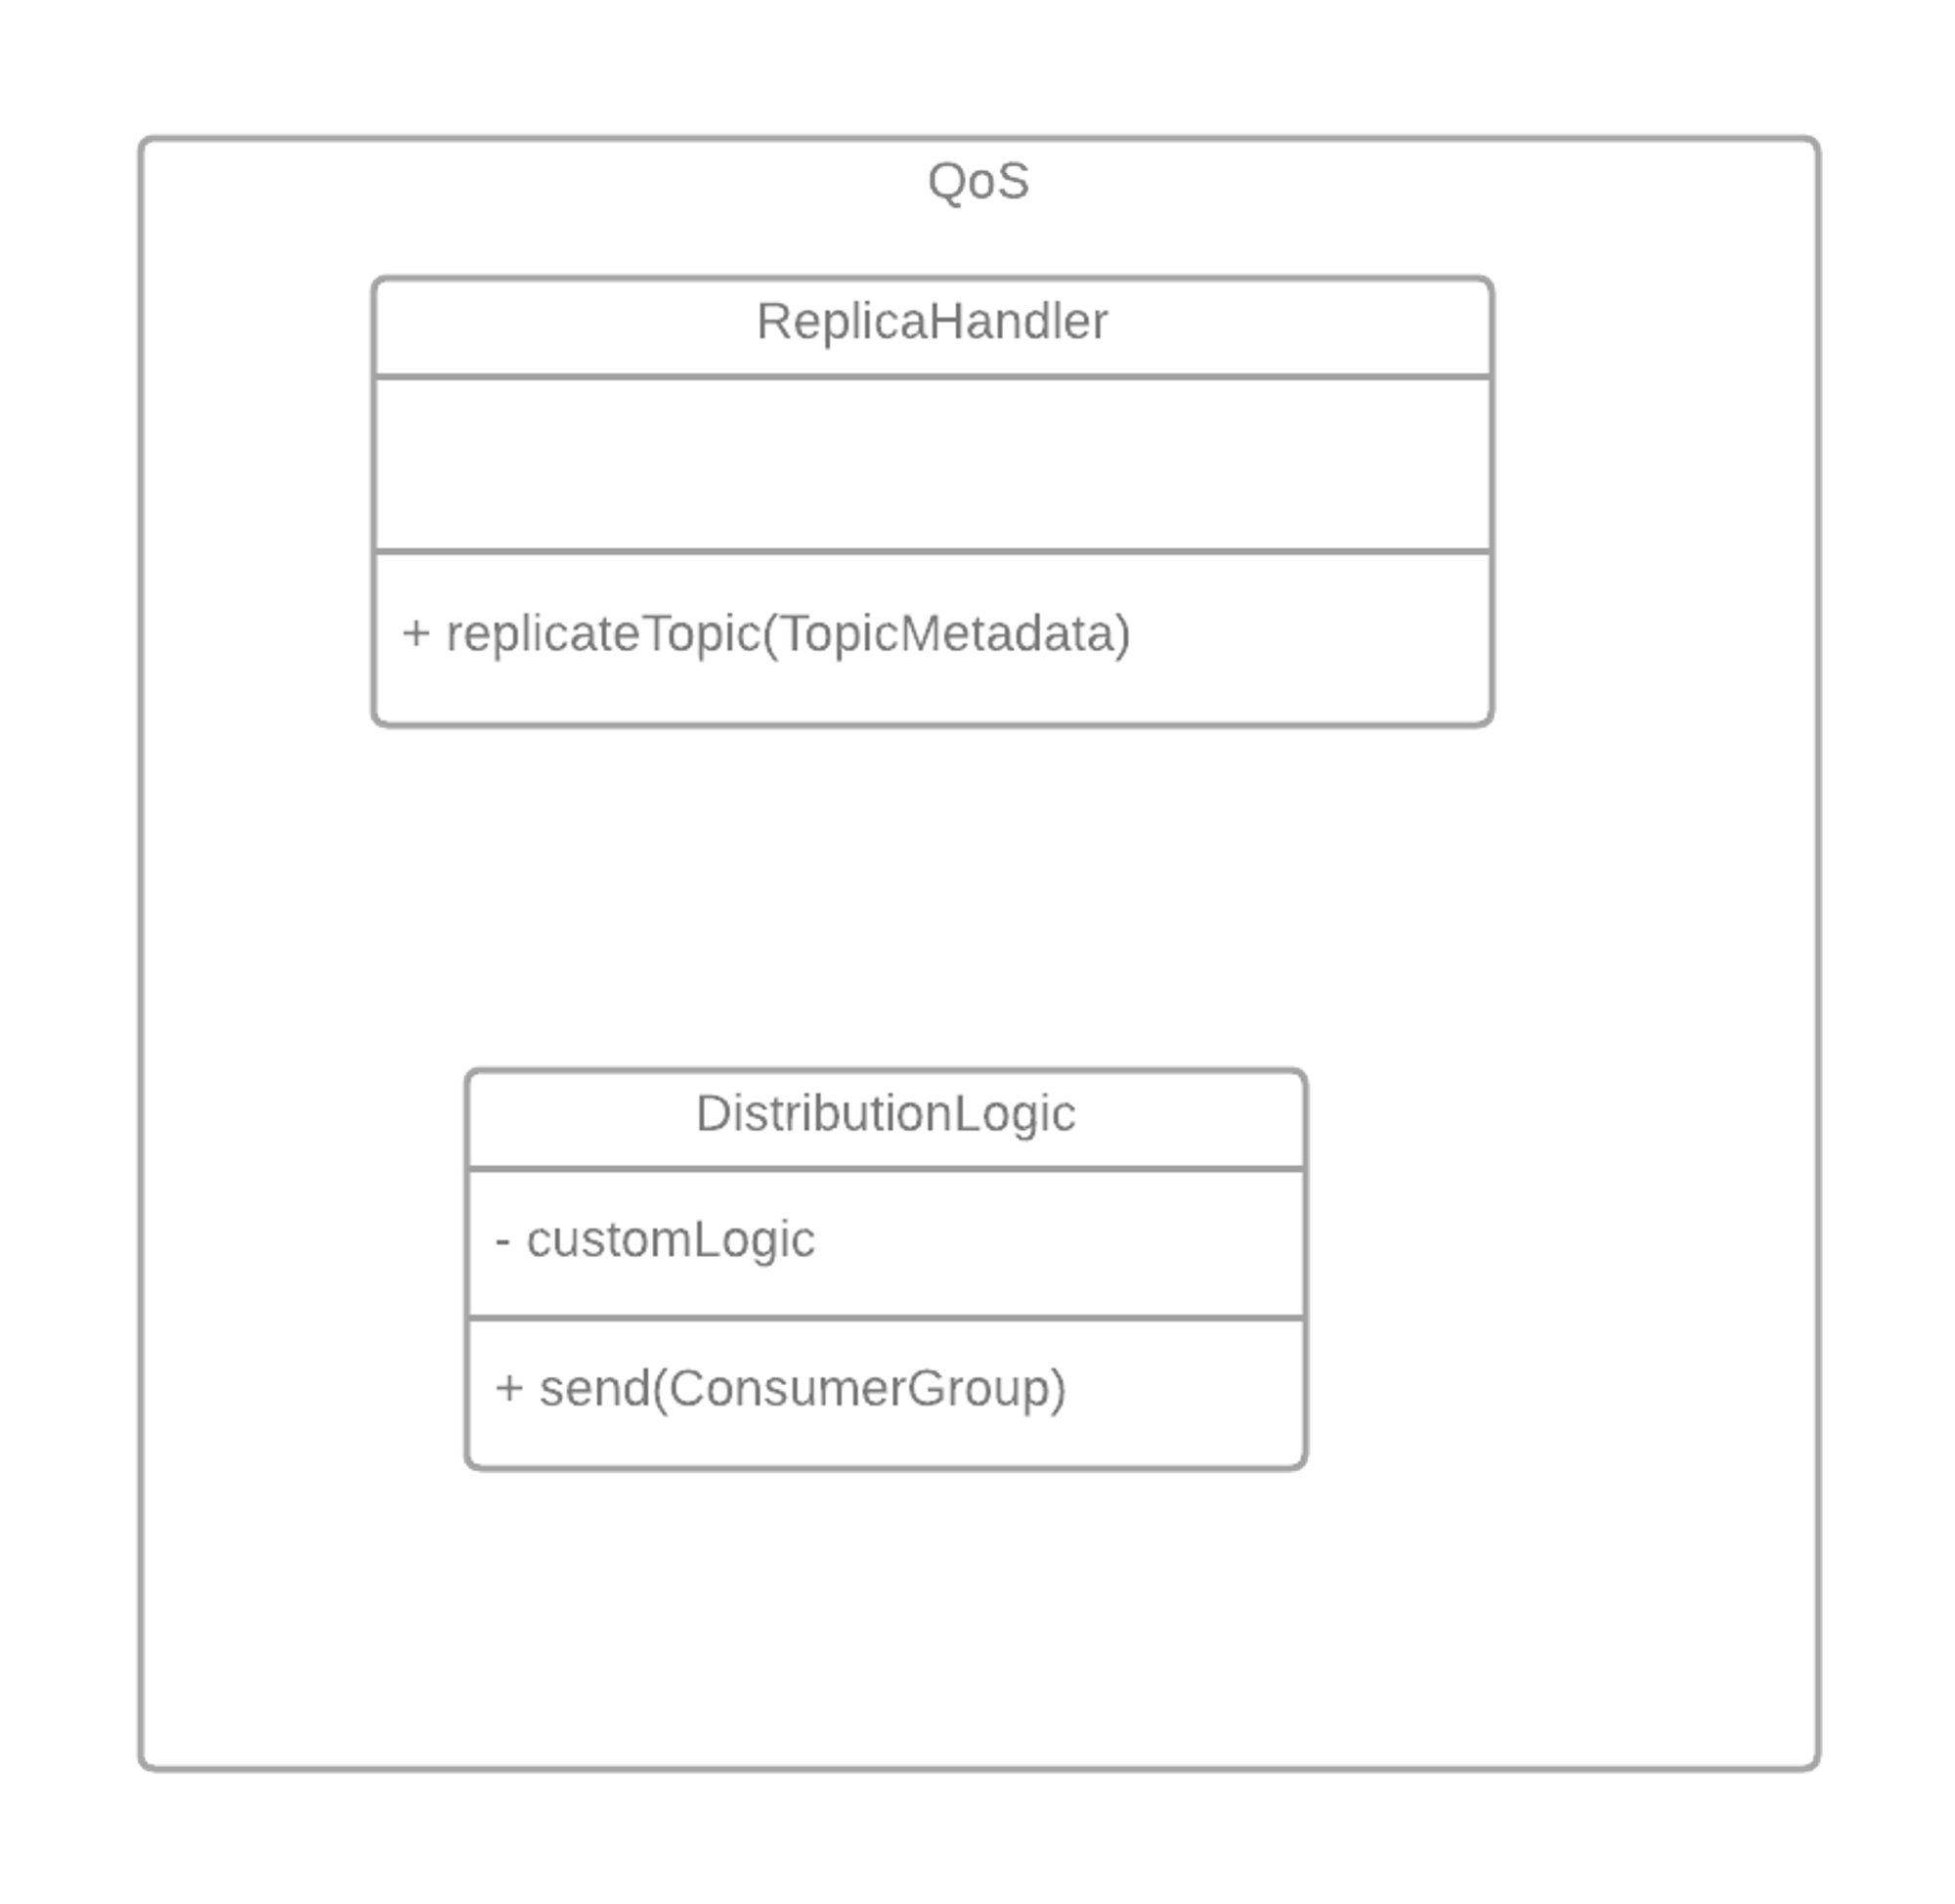
\includegraphics[width=0.7\textwidth]{Figures/class_diagram_QoS.png}
    \caption{Class diagram of the QoS layer}
\end{figure}

The components are:

\begin{itemize}
    \item   ReplicaHandler: this component is used for replicating topics to
            ensure high availability and durability of data. It takes a
            TopicMetadata object as a paramater, which contains information
            about the topic to be replicated. The ReplicaHandler then
            replicates the topic to a specified number of brokers.
    \item   DistributionLogic: this component is responsible for distributing
            messages to consumer groups in a way that meets the QoS
            requirements of the application. It takes a ConsumerGroup object
            as a paramter, which contains information about te consumers
            belonging to the group that has to be serviced.
            The DistributionLogic then distributes the messages to the consumer
            group in a way that ensures that all messages are eventually
            delivered to at least one consumer.
\end{itemize}

The QoS layer has the necessity to interact with other elements of the system
in order to work. In particular, the complexity of the above layer, the topic
manager, gives the possibility to simplify this layer, which will exploits
the classes given by the communicaiton layer to perform the exchange of
messages in a simple way.

\subsection{Communication}

The communication layer is responsible for sending and receiving messages
between the processors in the system and outside of the embedded system.
The layer is one of the most important ones in the domain of a
platform for pub/sub communication. This layer takes into consideration the
necessity for embedded system of using restrained resources.

\begin{figure}[H]
    \centering
    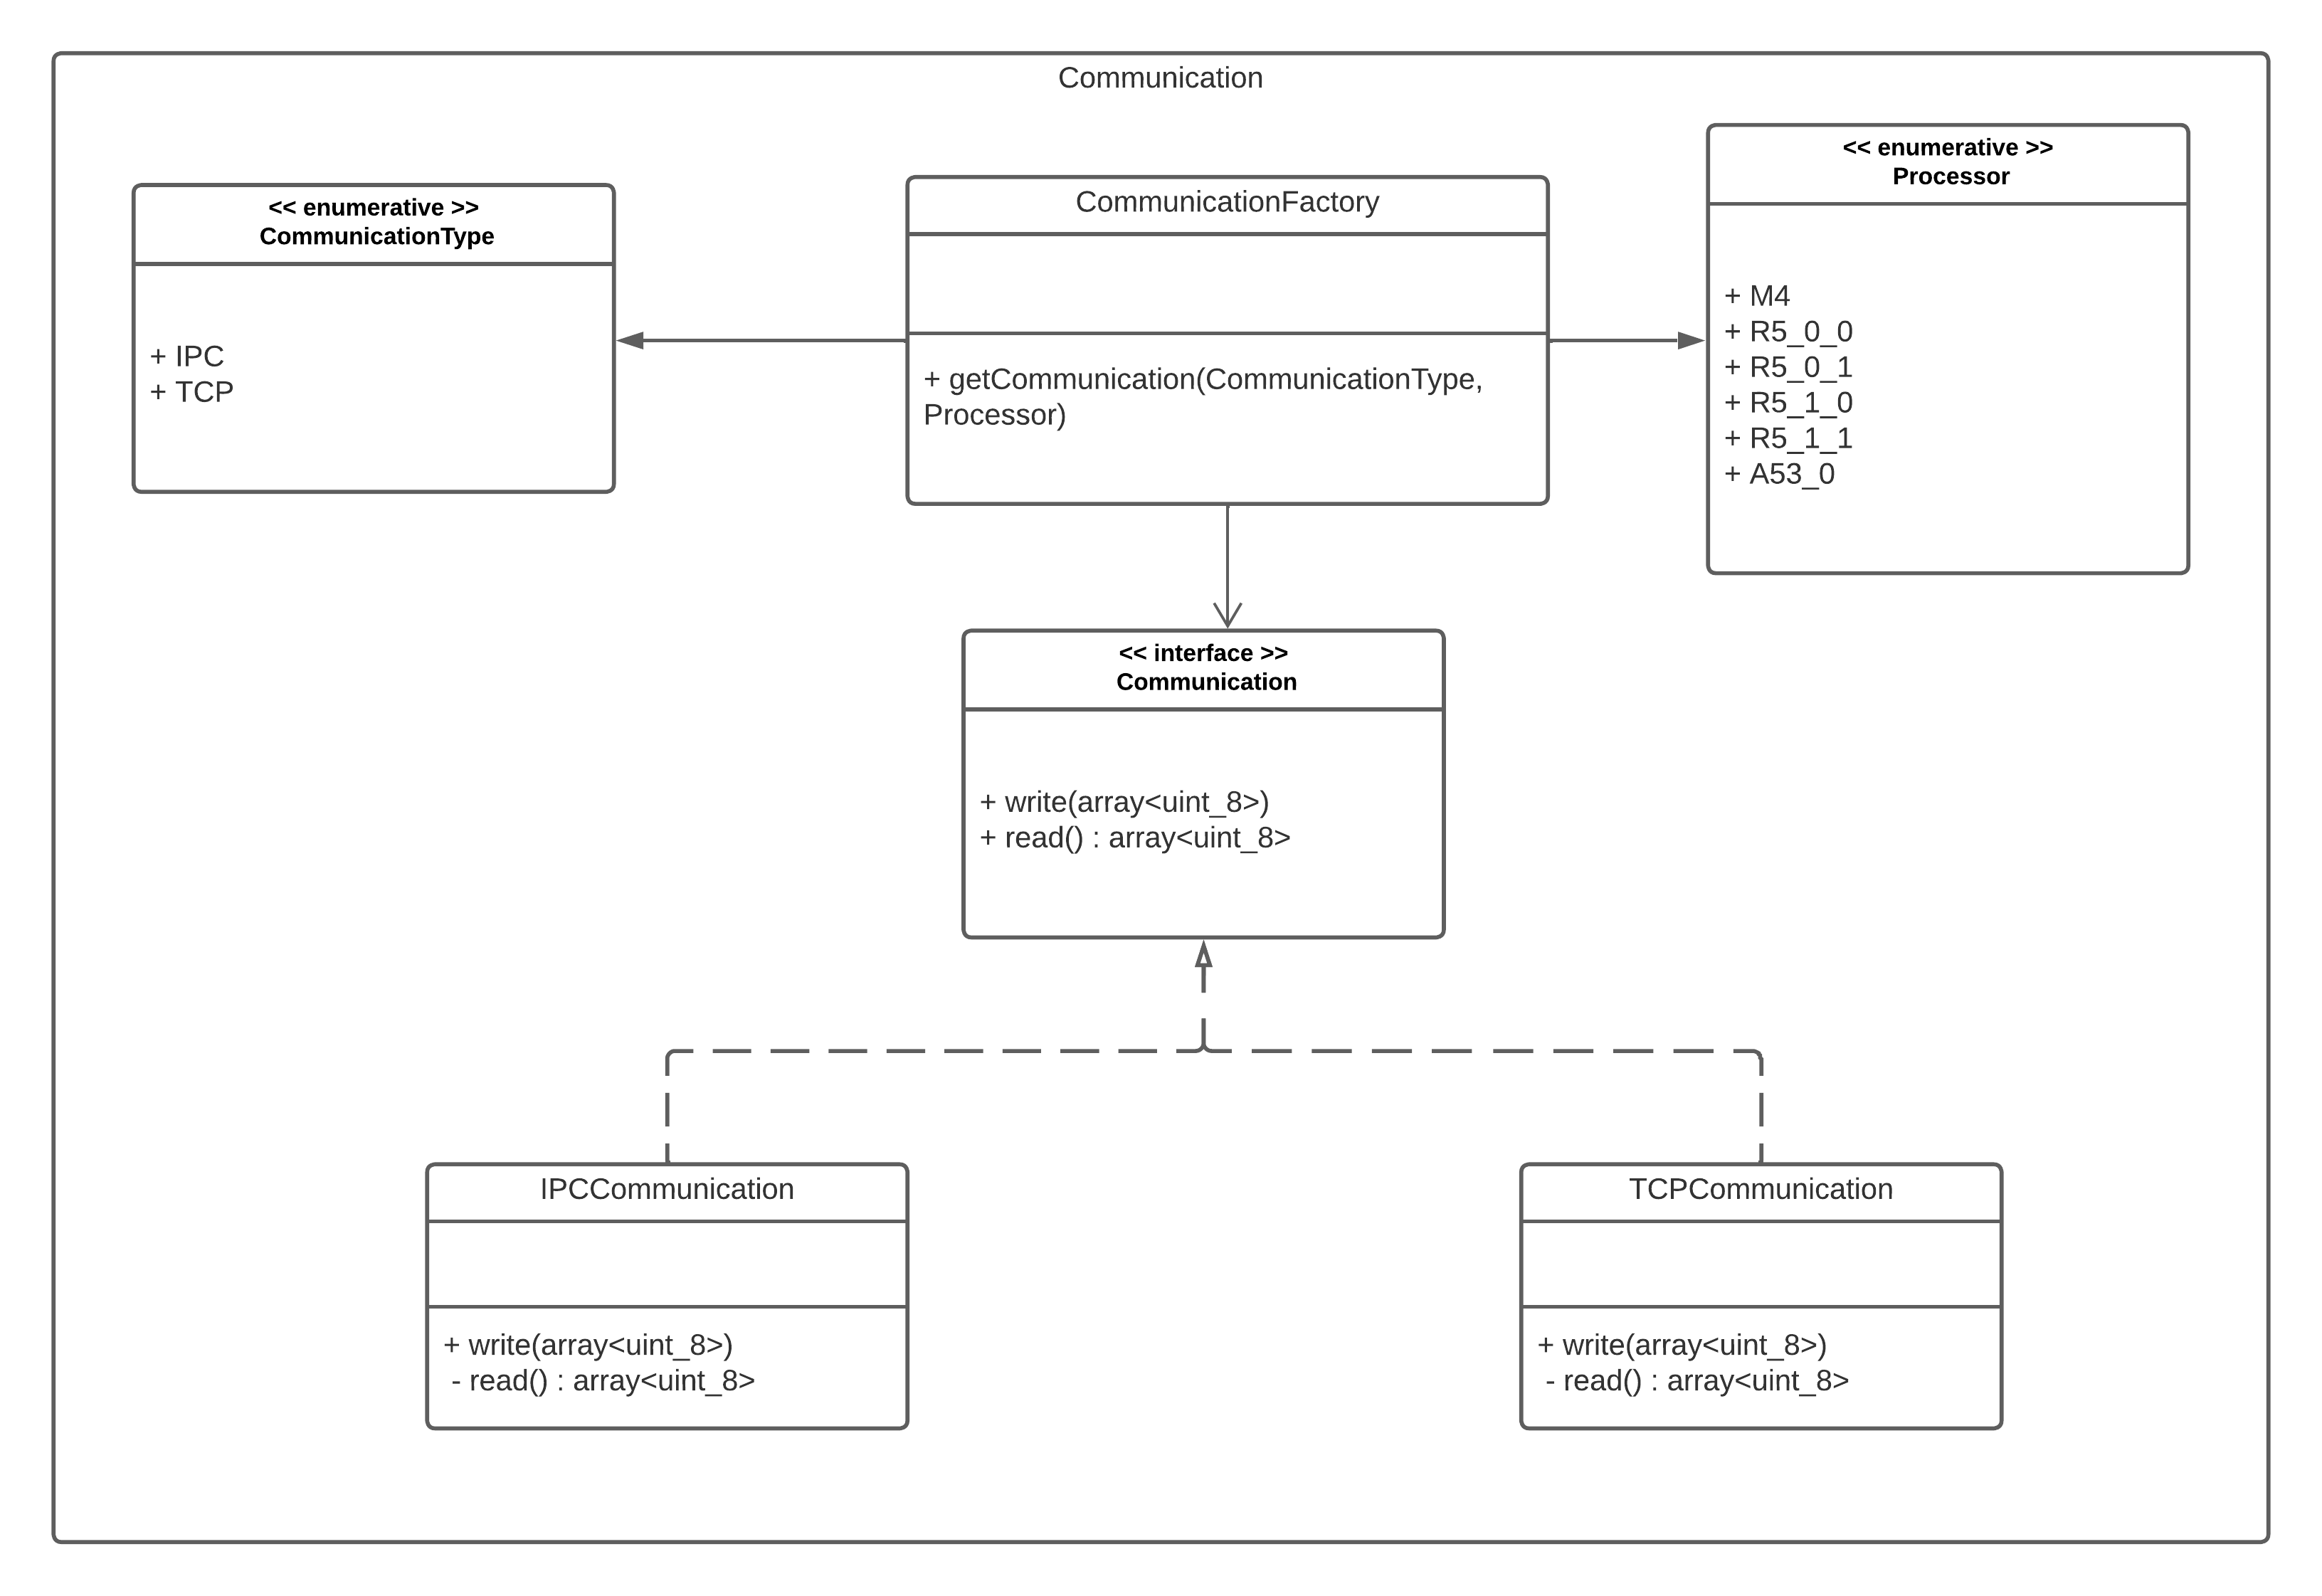
\includegraphics[width=1.0\textwidth]{Figures/class_diagram_communication.png}
    \caption{Class diagram of the communication layer}
    \label{fig:class_diagram_communication}
\end{figure}

The components seen in the class diagram
(figure \ref{fig:class_diagram_communication}) are:

\begin{itemize}
    \item   CommunicationFactory: this class is responsible for creating
            instances of IPCCommunication or TCPCommunication objects. It takes
            a CommunicationType parameter.
    \item   CommunicationType: this enumeration defines the two types of
            communication that cna be created: IPC or TCP.
    \item   IPCCommunication: This class is used for communication between
            processors on the same device. It provides methods for sending and
            receiving messages.
    \item   TCPCommunication: this class is used for communication between
            processors on different devices. it provides methods for sending
            and receiving messages over a TCP socket.
\end{itemize}

\subsection{Domain level}

The image below (figure \ref{fig:class_diagram_domain}) shows all the classes
that compose the domain of the system.
The domain classes can be used by all the layer of the application (primarly
from the top level layers) and they contain information of the specific class
and the interaction with the other elements.

\begin{figure}[H]
    \centering
    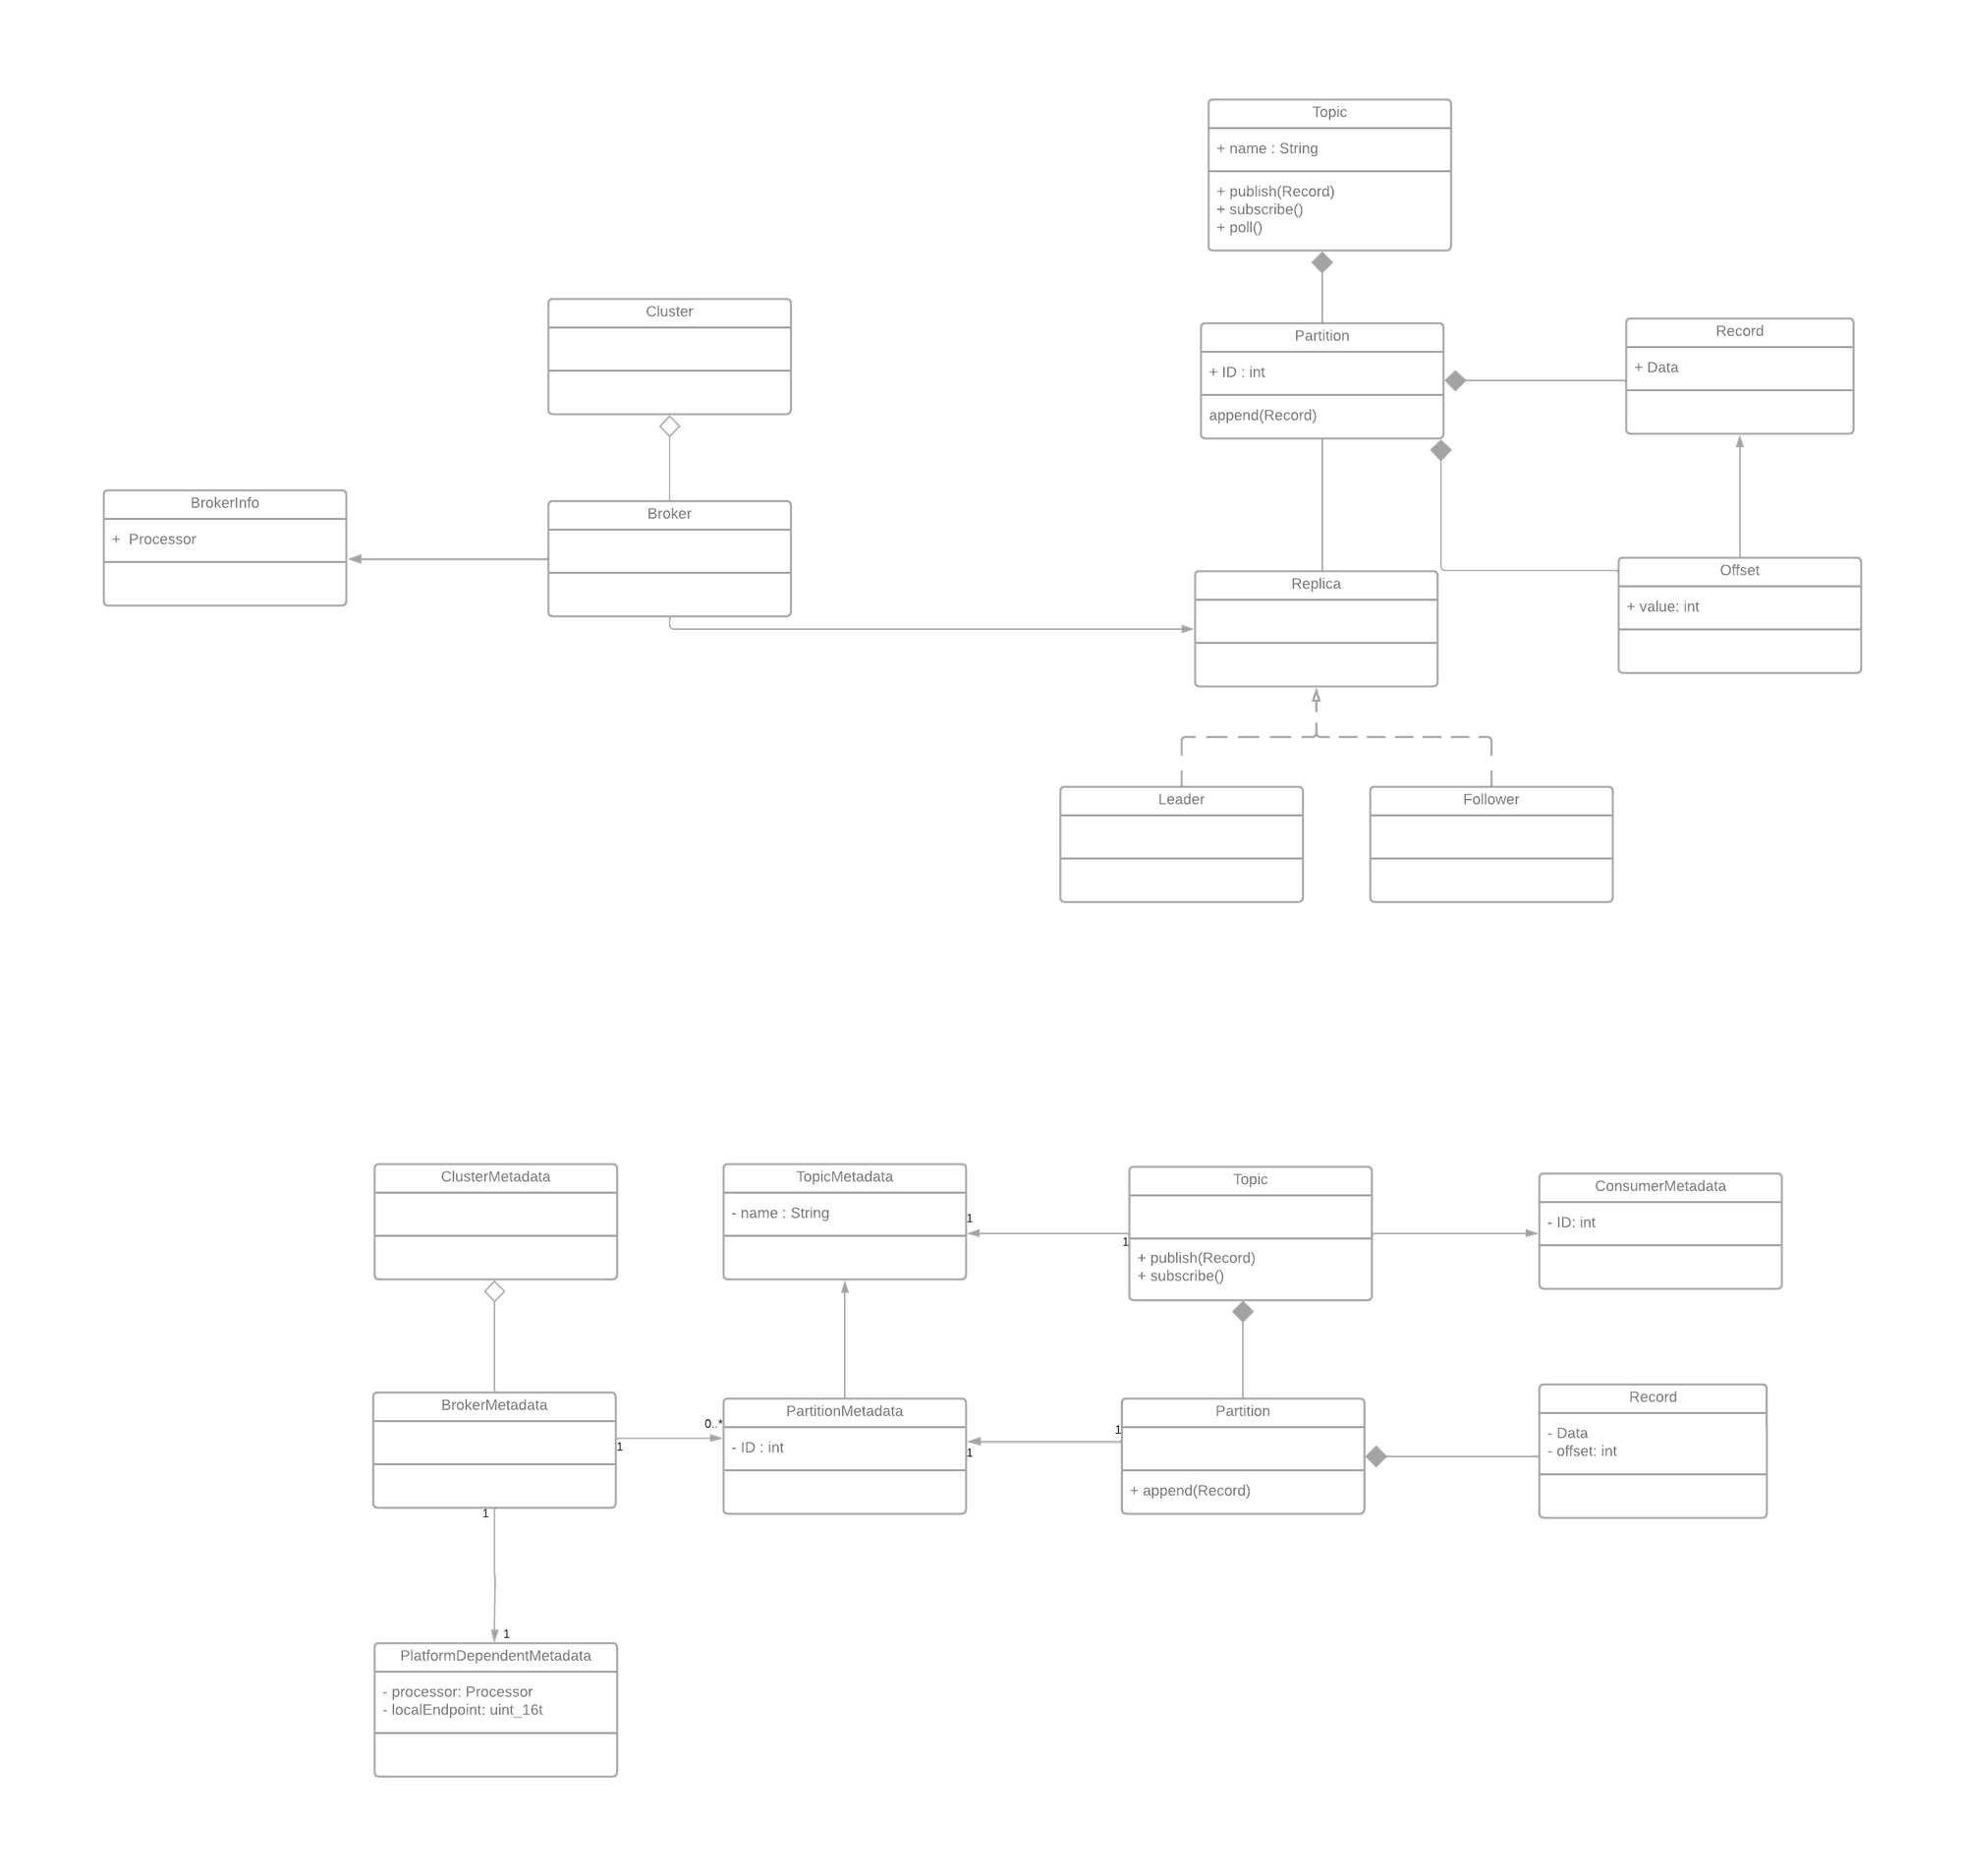
\includegraphics[width=1.0\textwidth]{Figures/class_diagram_domain.png}
    \caption{Class diagram of domain of the middleware}
    \label{fig:class_diagram_domain}
\end{figure}

\section{Sequence Diagram}

The following section will use sequence diagrams to visualize the steps needed 
and the classes interaction to perform the most important operations of the
system.

\subsection{Consumer asking for a record}

The sequence diagram depicts the interaction between a message consumer and
the rest of the system. The consumer initiates the interaction by requesting
a TopicProxy from the TopicFactory.
The patter proxy helps to hide all the operations that will be done underneath
to perfrom the commuincation between the different processors, making it seem
like a local communication.
The consumer then establishes a communication channel with the broker
containing the interested topic using the CommunicationFactory.
The SystemManager is used to retrieve the information about the cluster status.

\begin{figure}[H]
    \centering
    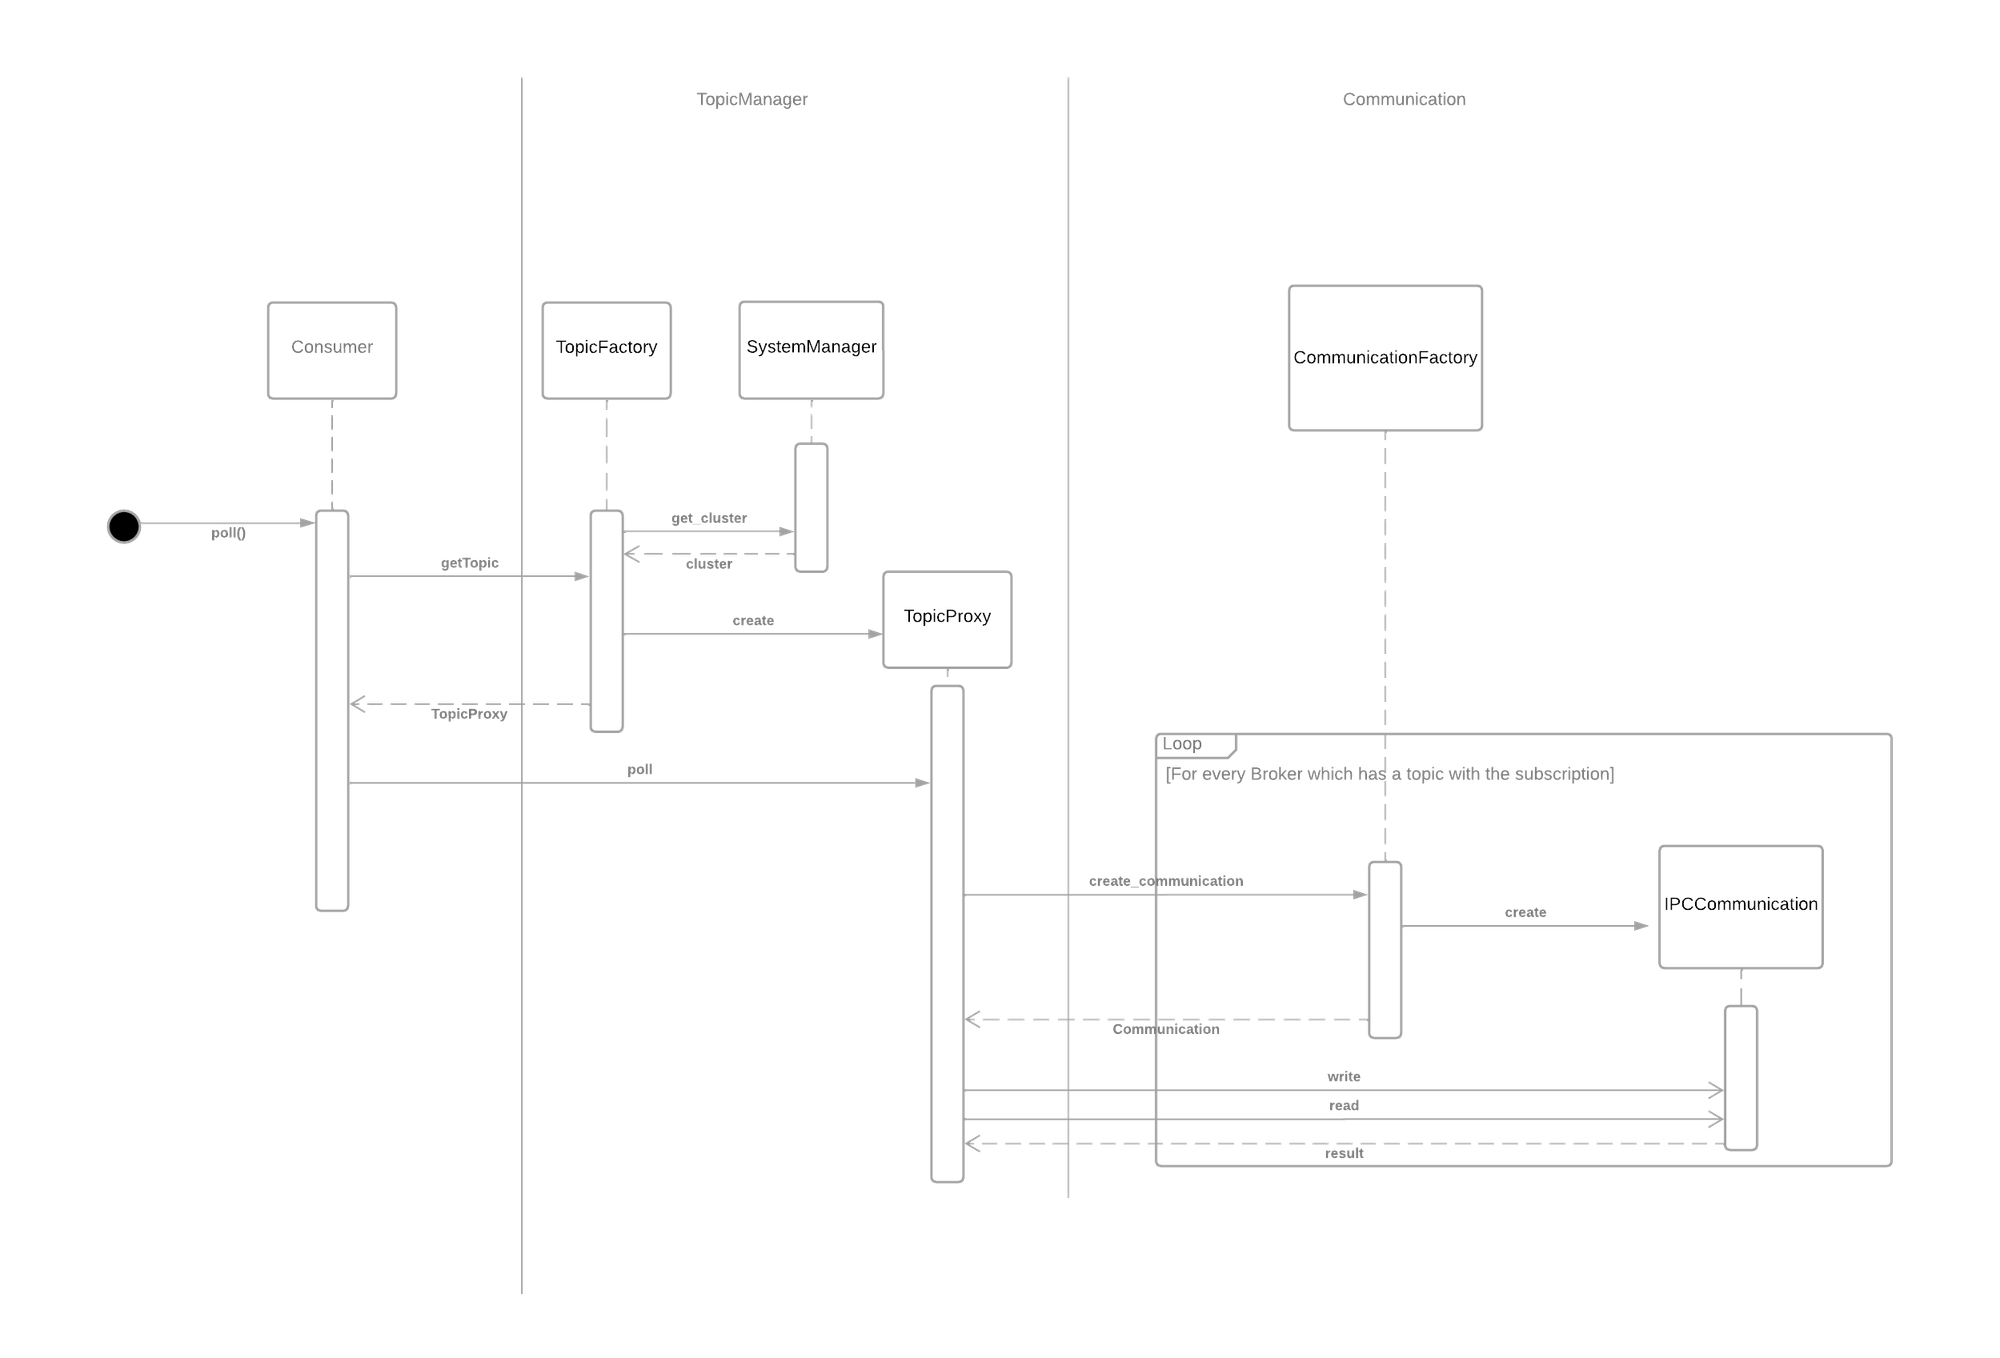
\includegraphics[width=1.0\textwidth]{Figures/sequence_diagram_consumer_poll.png}
    \caption{Sequence diagram of a consumer asking for a record}
\end{figure}

\subsection{Publisher sending a record}

The publishing of a message is handled in a similar way to the consumer read.
All the details is hidden under the TopicProxy and the SystemManager.

\begin{figure}[ht]
    \centering
    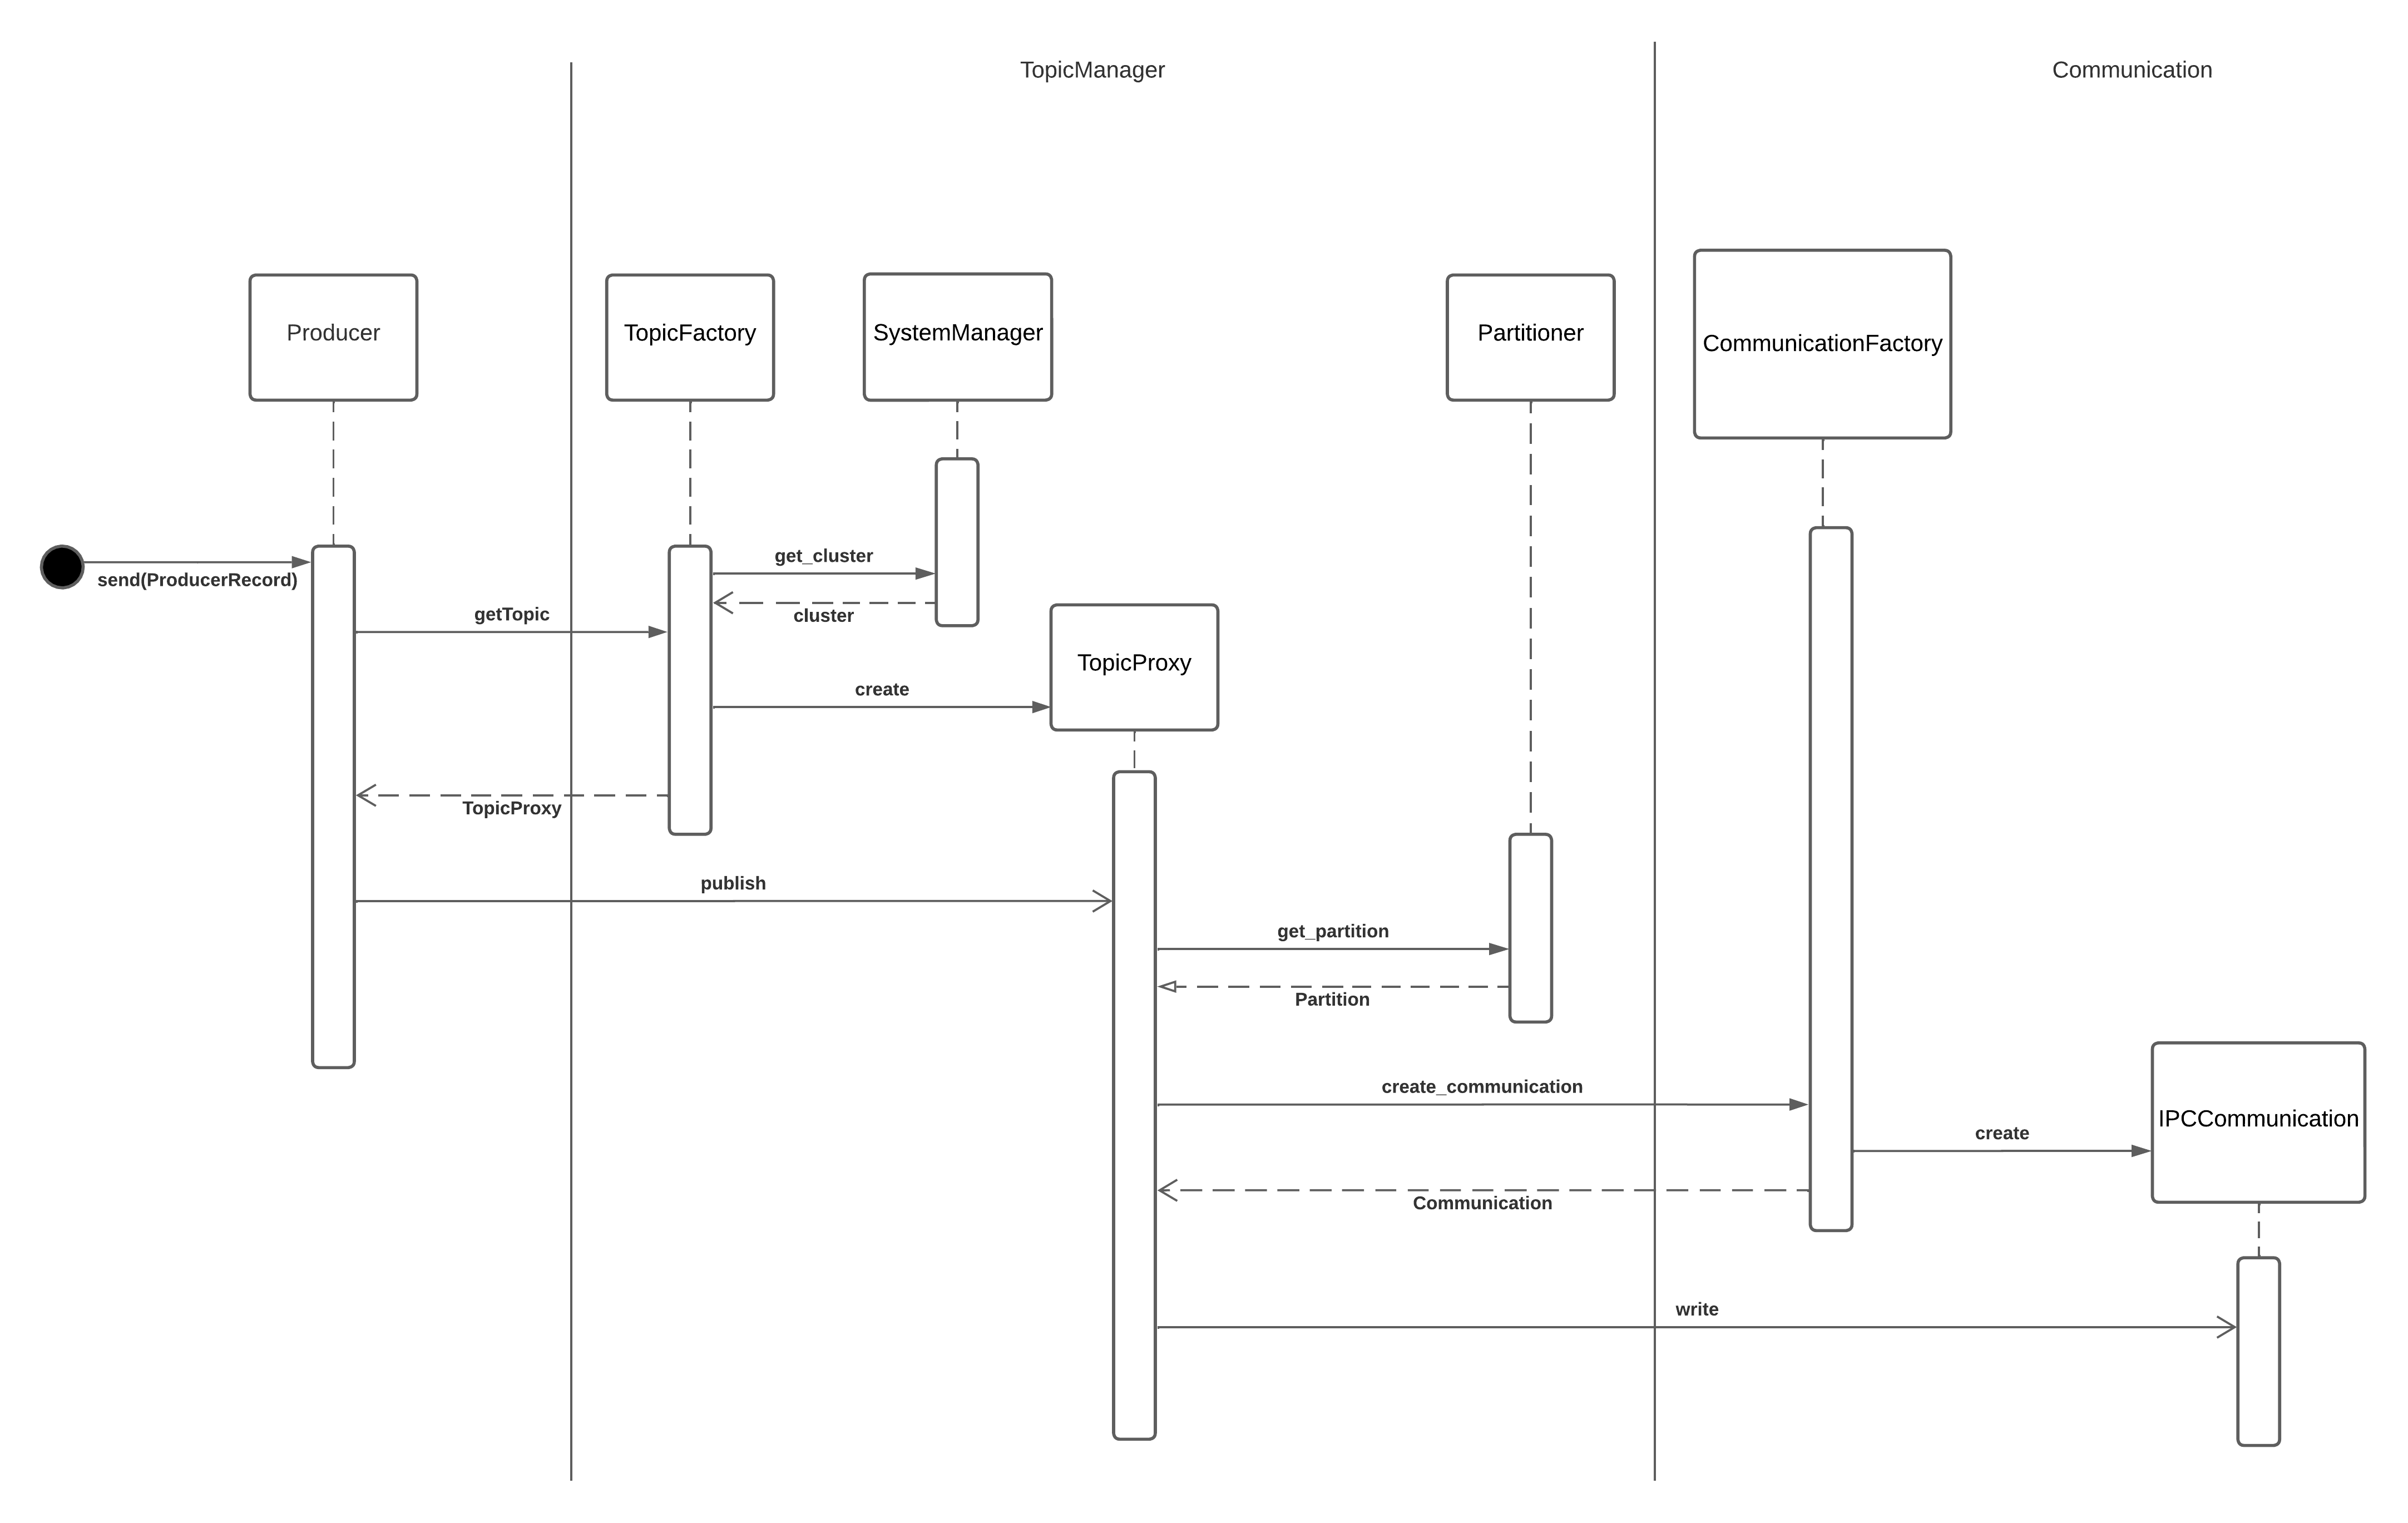
\includegraphics[width=1.0\textwidth]{Figures/sequence_diagram_producer.png}
    \caption{Sequence diagram of a producer publishing a record}
\end{figure}

\subsection{Synchronization of the cluster status}

The synchronization of the cluster status is a fundamental operation in a
distributed system.
The operation is divided in two steps:

\begin{enumerate}
    \item   The first one is performed by the system manager to ask to the
            centralized "server" (configurer) about the information. 
    \item   The second one is performed by the configurer which responds to
            the request sent by the system manager.
\end{enumerate}

\begin{figure}[H]
    \centering
    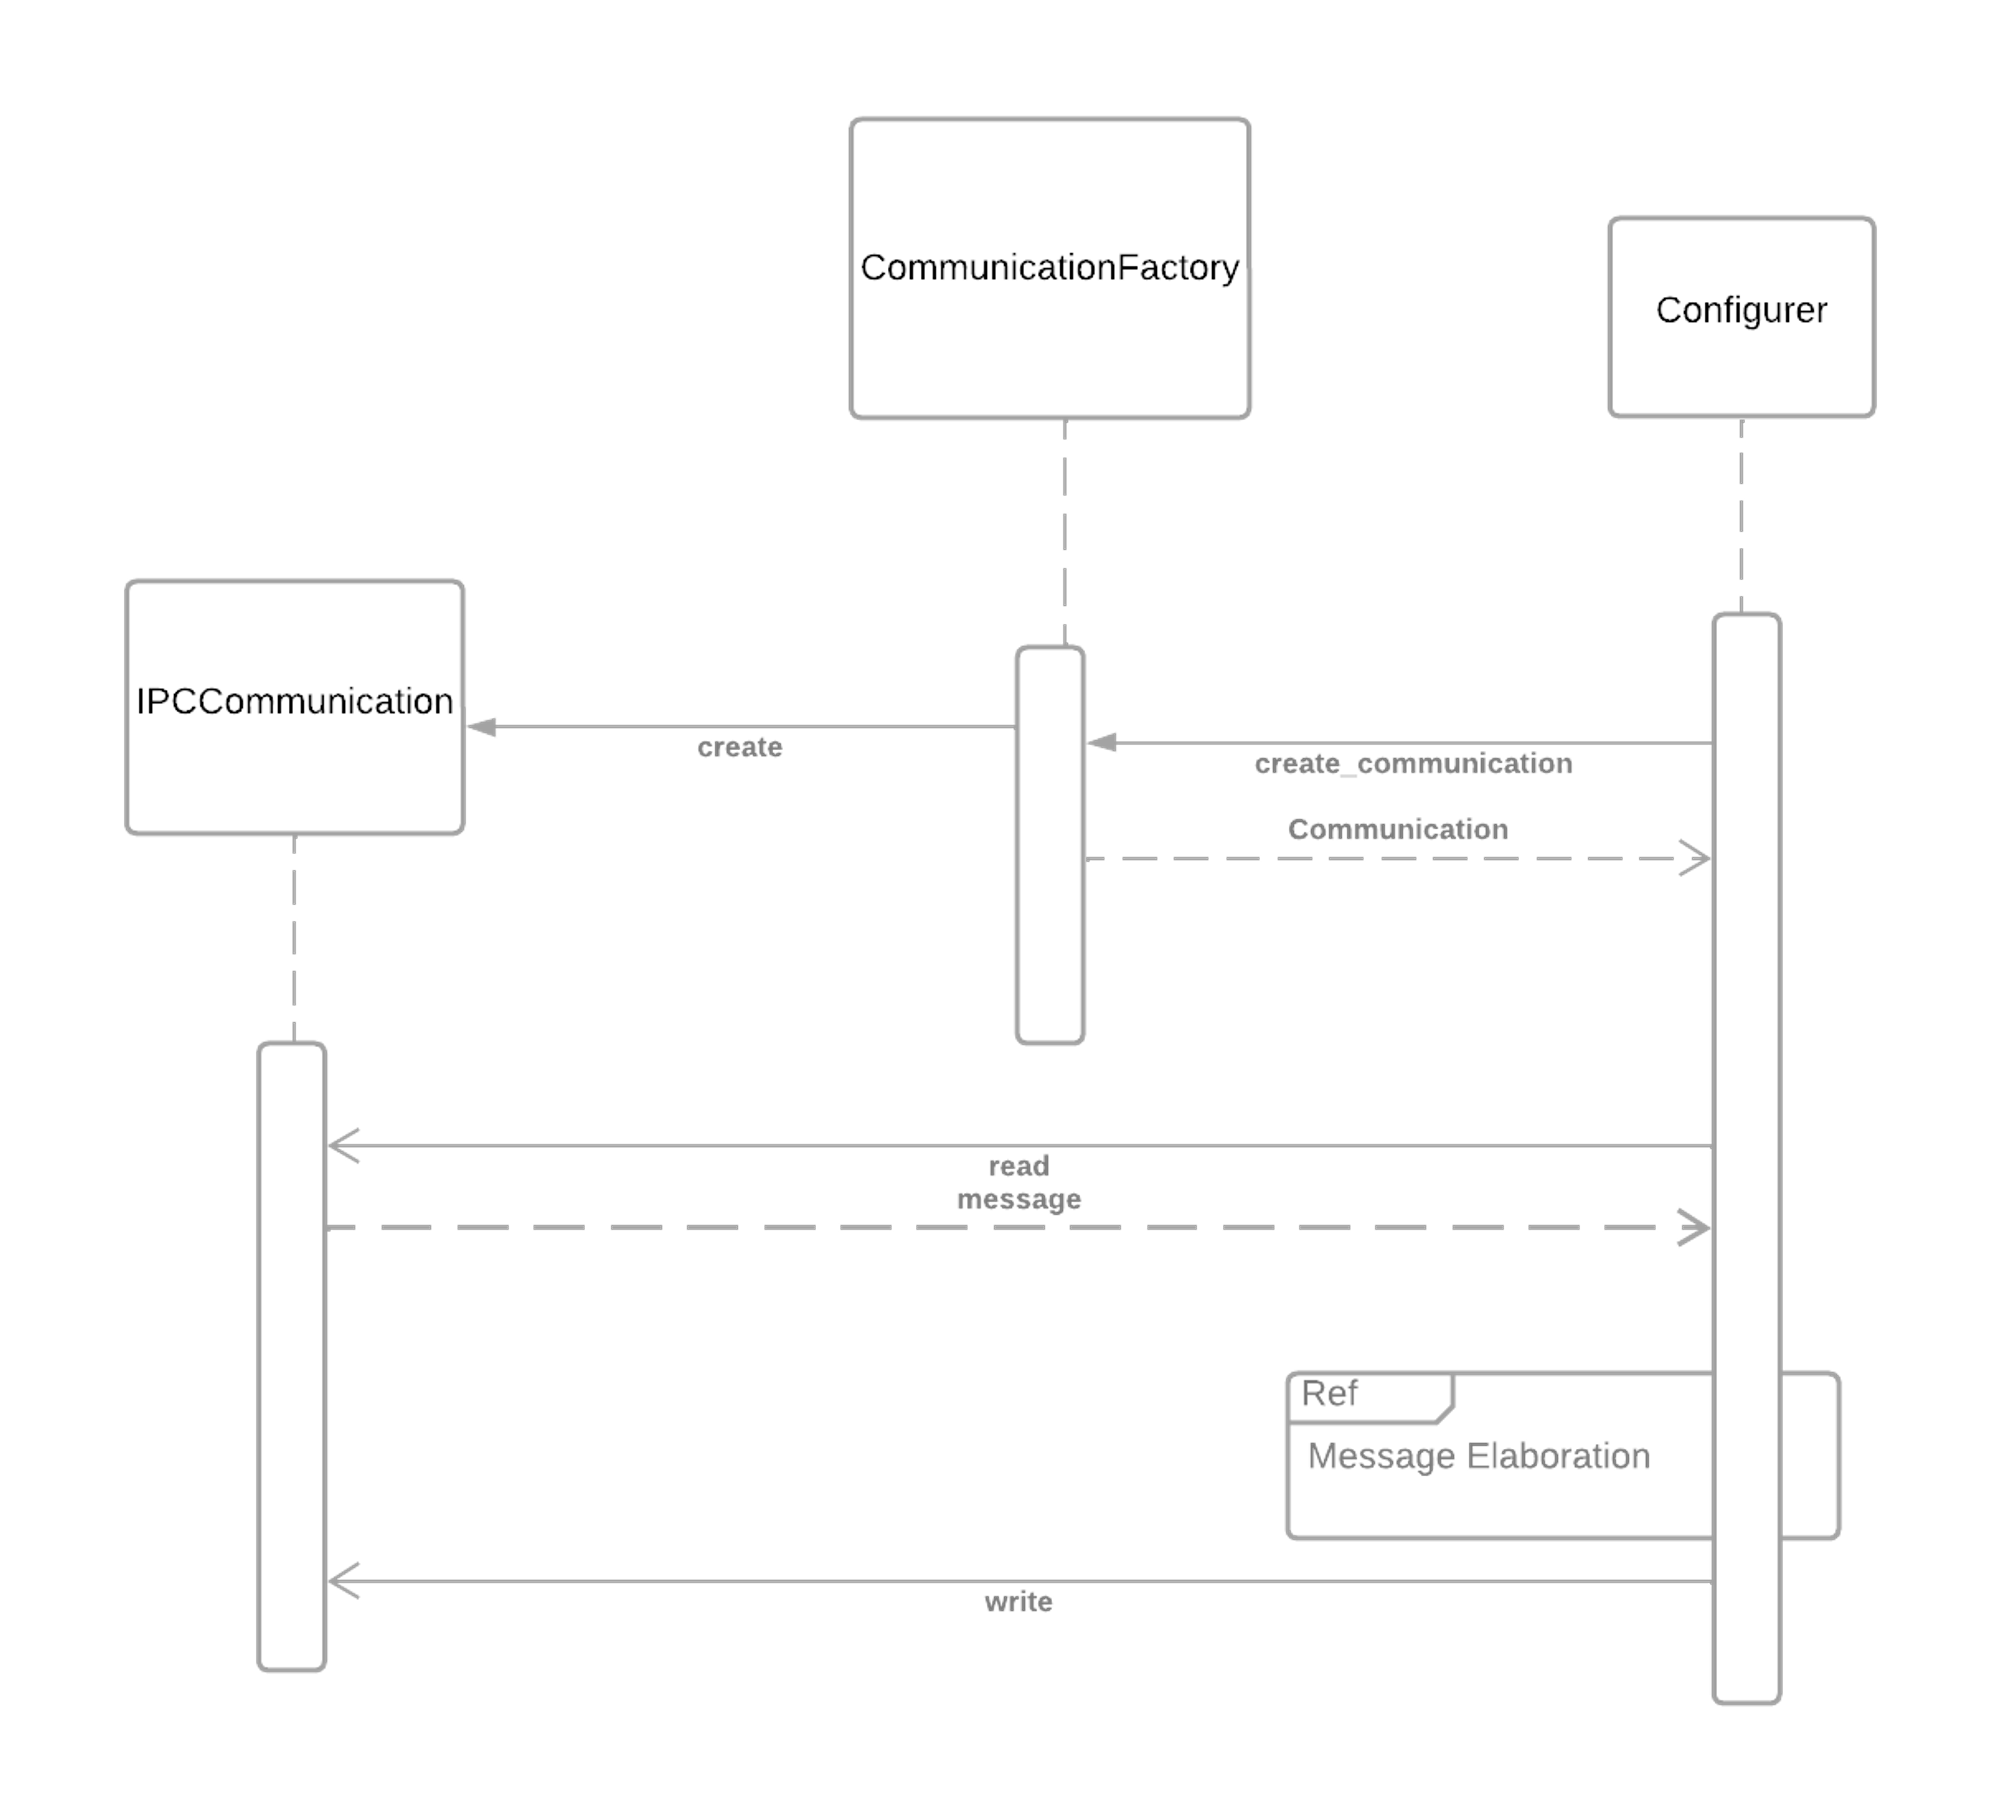
\includegraphics[width=0.7\textwidth]{Figures/sequence_diagram_cluster_status_configurer.png}
    \caption{Sequence diagram of the configurer operations done for the cluster
             status synchronization}
\end{figure}

\begin{figure}[H]
    \centering
    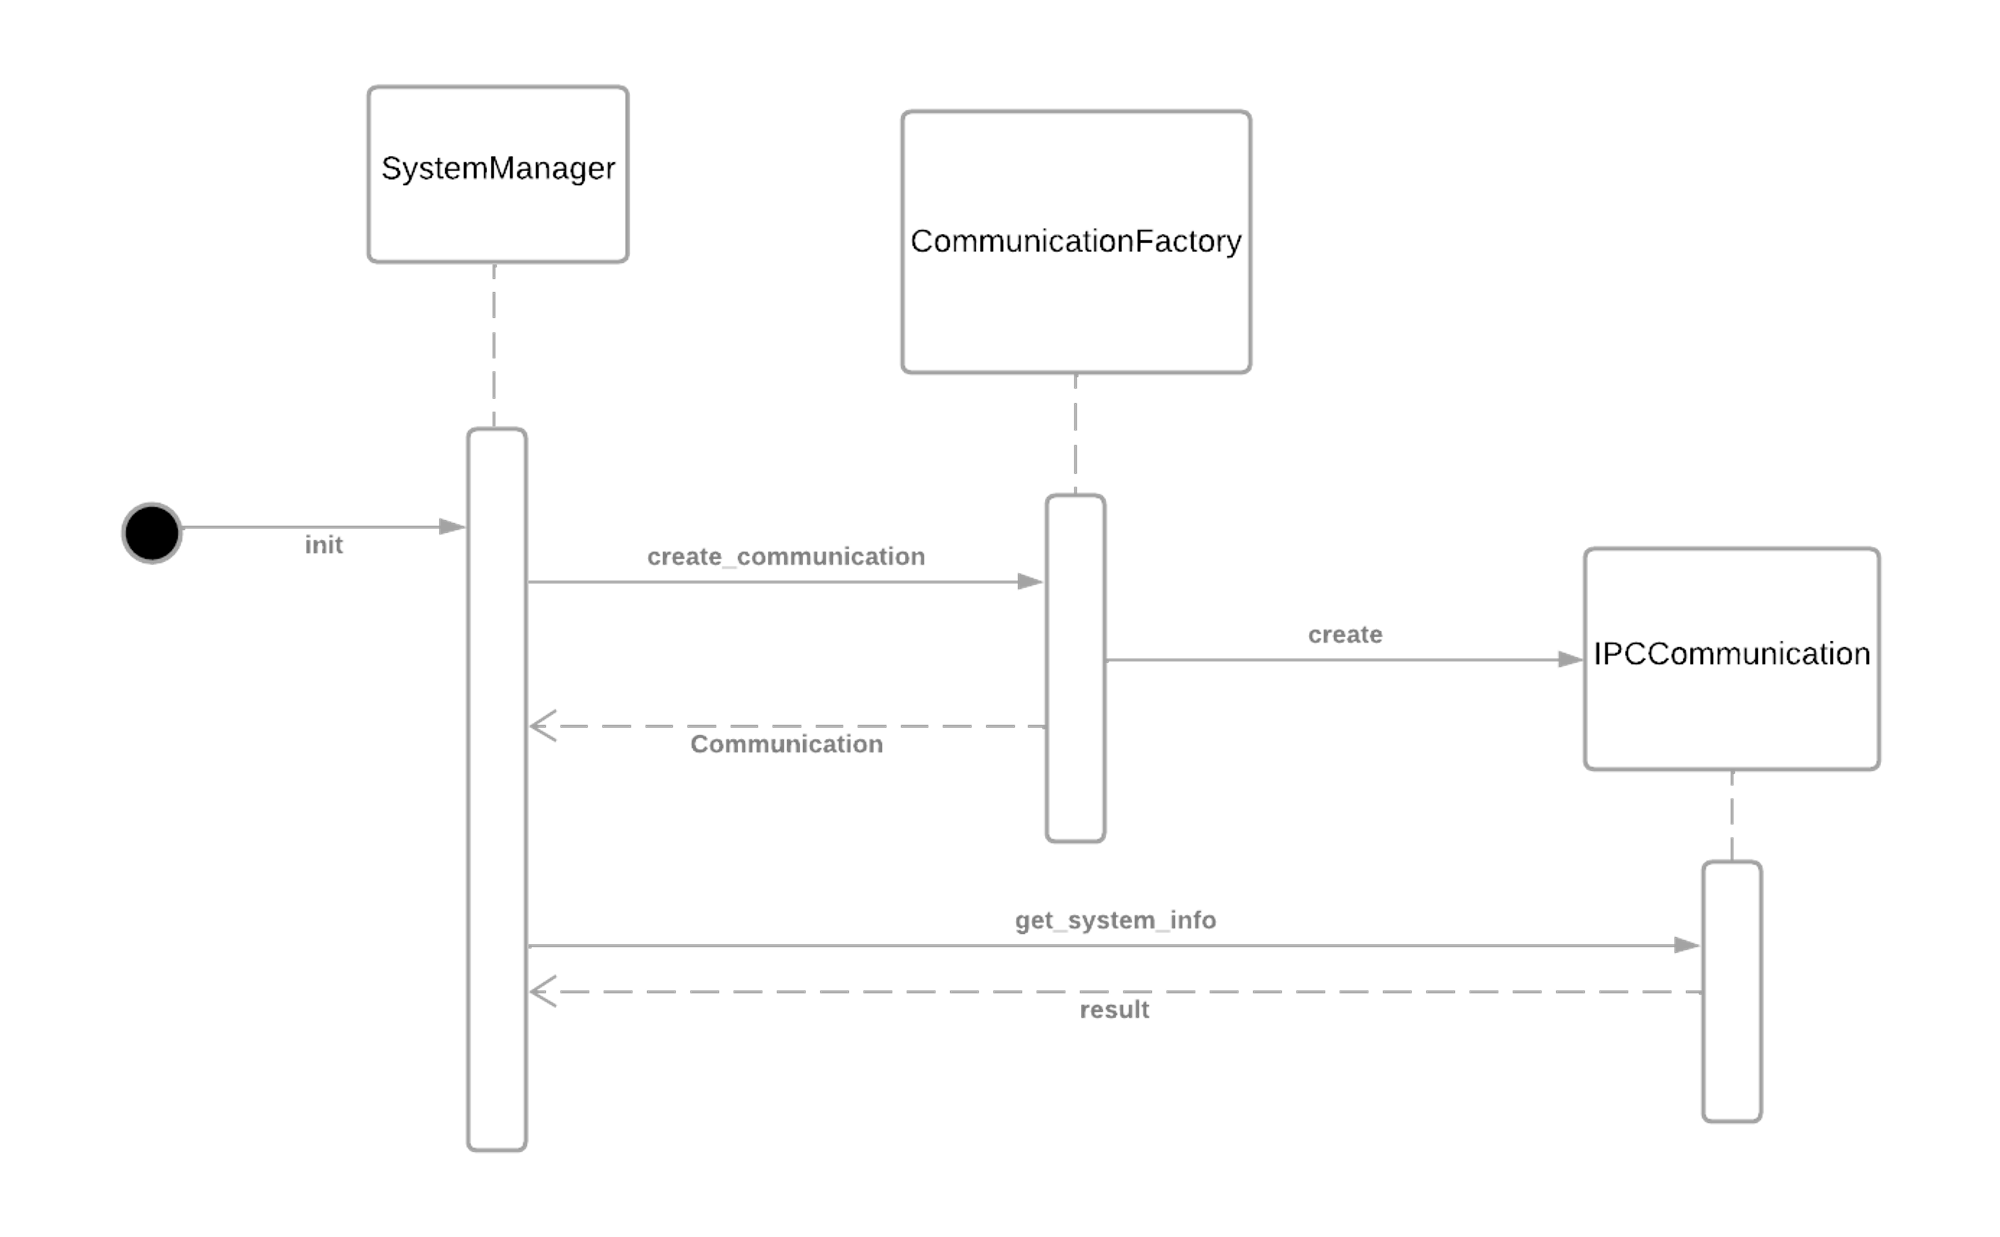
\includegraphics[width=0.7\textwidth]{Figures/sequence_diagram_cluster_status_system_manager.png}
    \caption{Sequence diagram of the system manager operations done for the
             cluster status synchronization}
\end{figure}

\subsection{Broker receiving a record}

One of the most important operation is the possibility to store the records,
sent by the producers, in a broker. 

\begin{figure}[H]
    \centering
    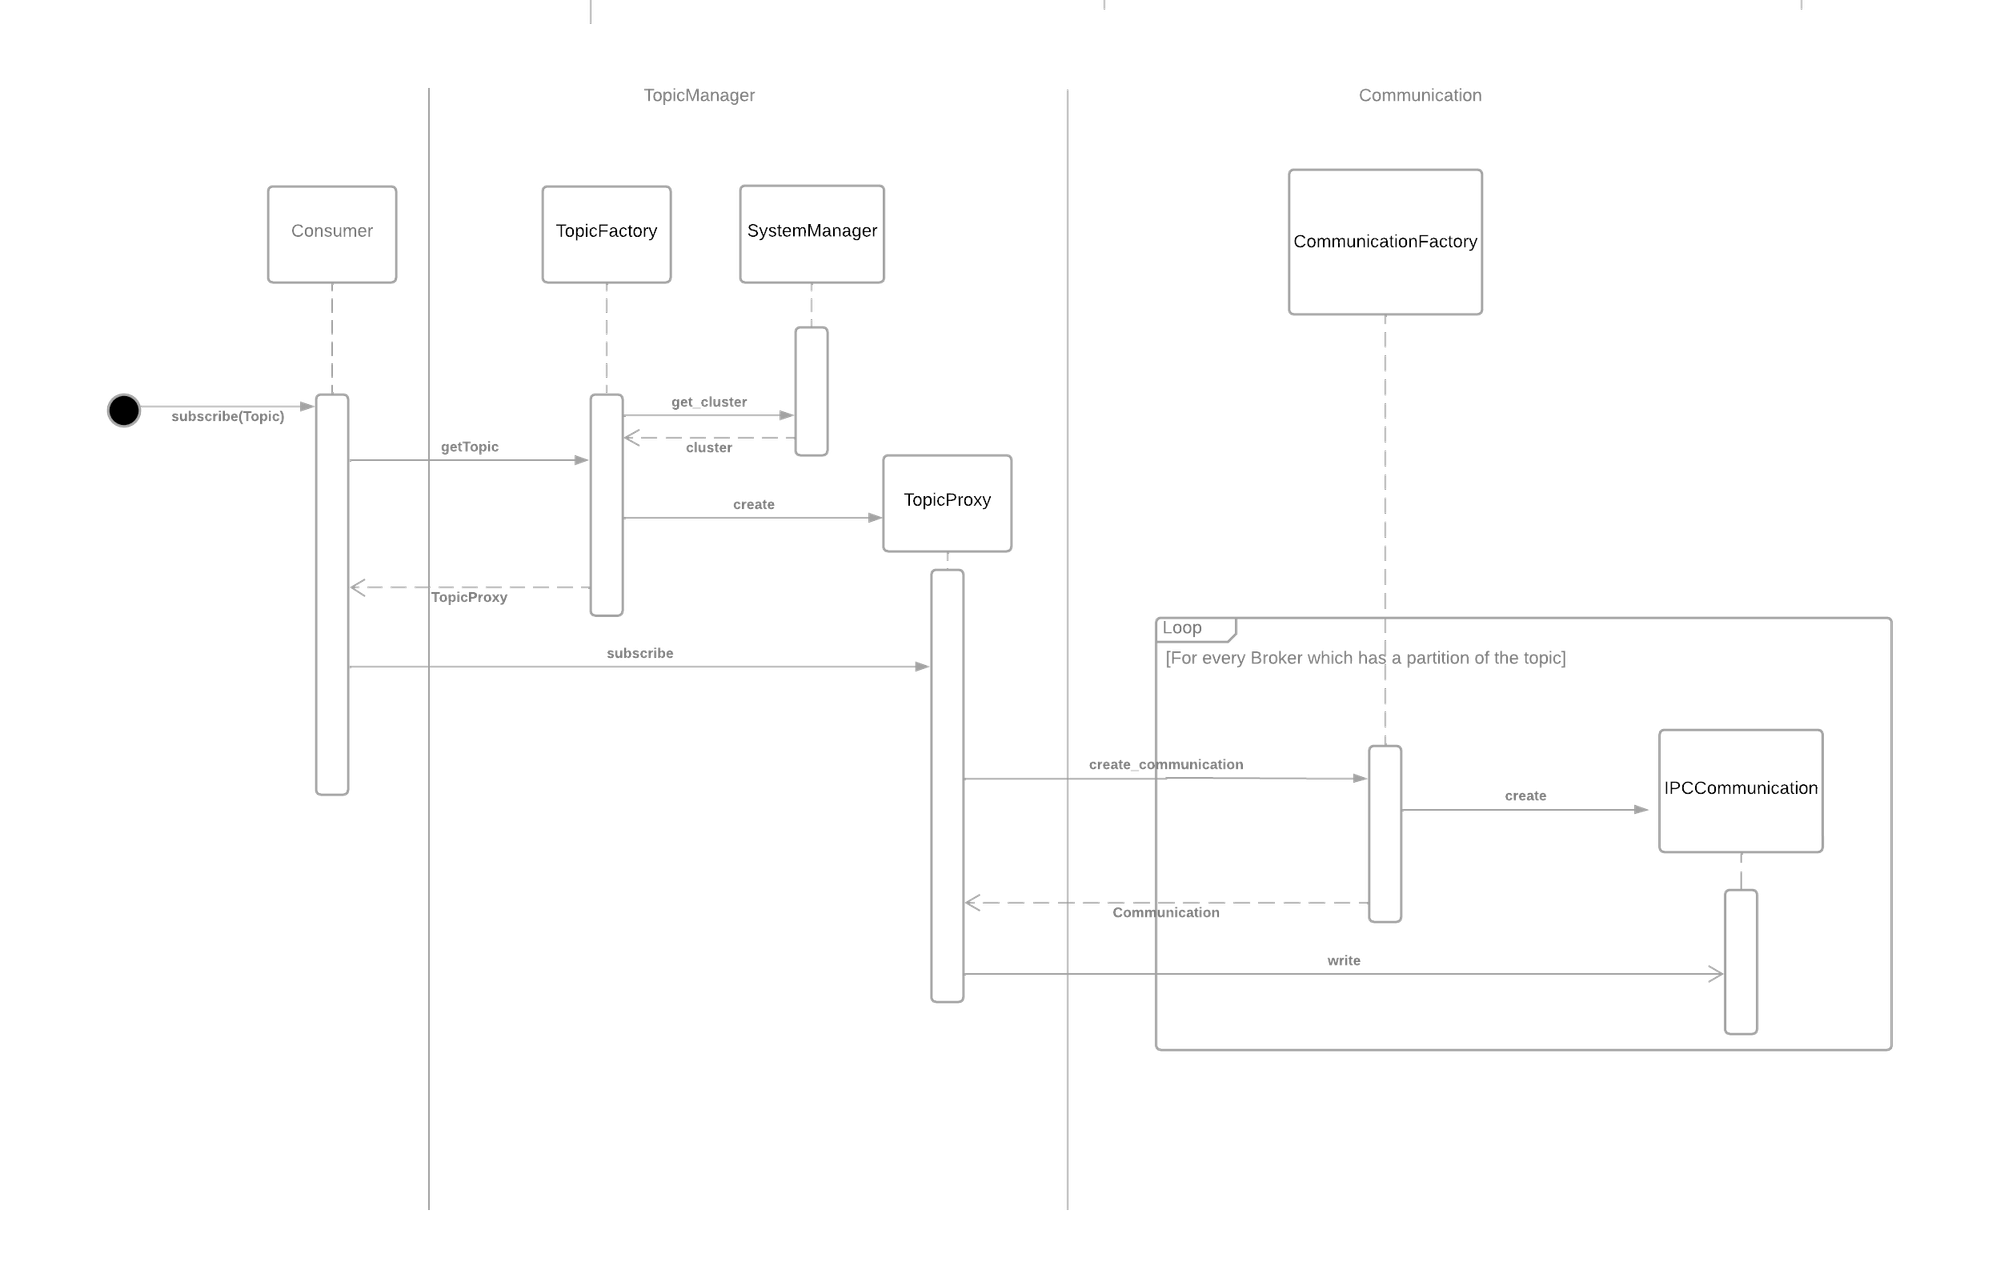
\includegraphics[width=1.0\textwidth]{Figures/sequence_diagram_broker.png}
    \caption{Sequence diagram of a broker receiving a record to store}
\end{figure}

\subsection{Consumer subscribing to a topic}

The subscription process involves a consumer expressing its interest in a
specific topic, intiiating a series of interaction with the underlying system.
The Consumer class uses the usual TopicProxy to communicate with the broker
holding the needed topic.

\begin{figure}[H]
    \centering
    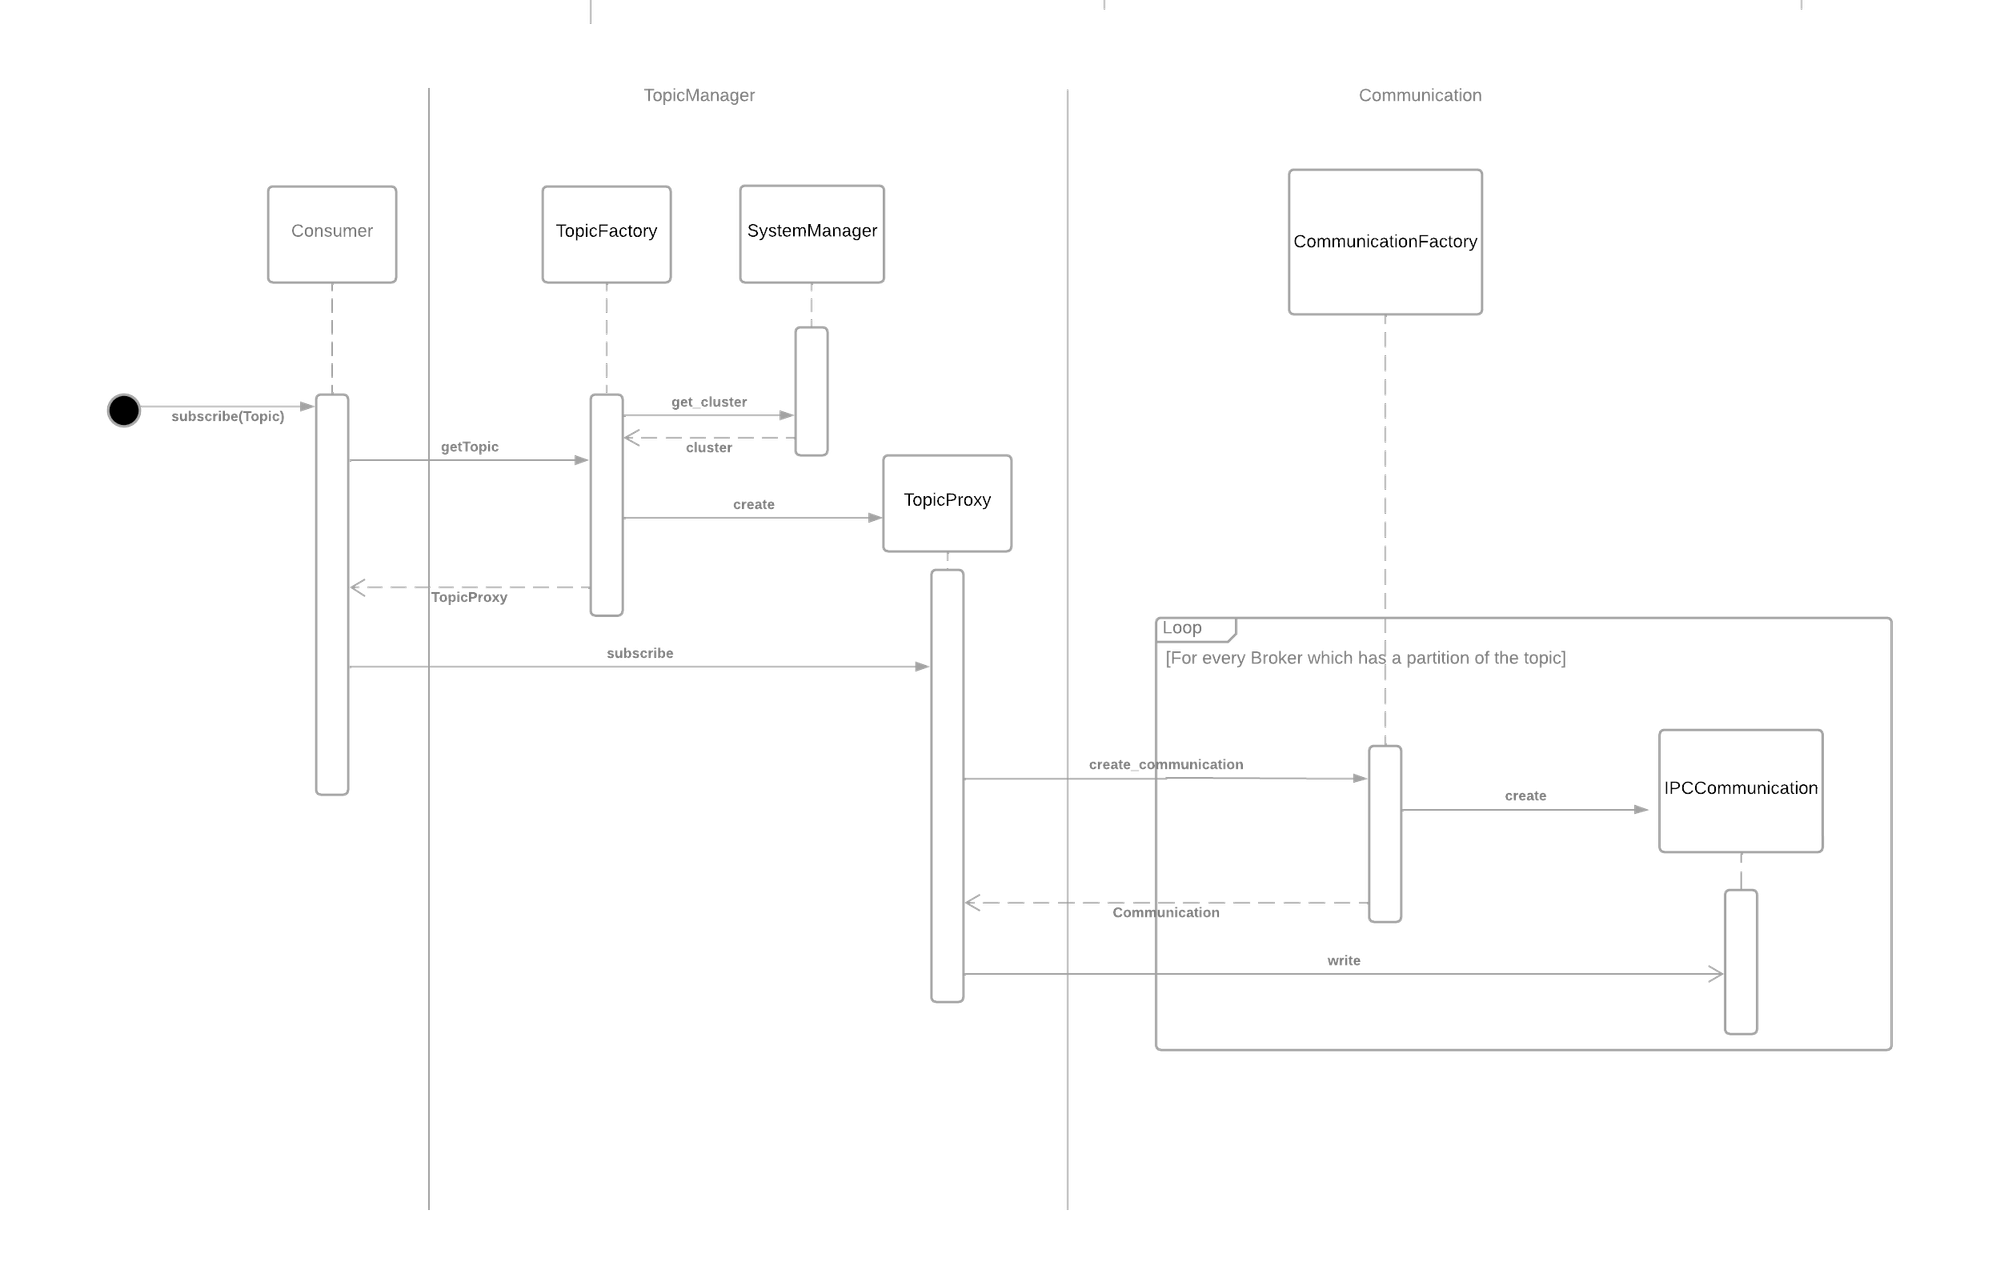
\includegraphics[width=1.0\textwidth]{Figures/sequence_diagram_subscription.png}
    \caption{Sequence diagram of a consumer subscribing to a topic handled by
             a broker}
\end{figure}


\section{Results}

The last phase of the project involved the development and performance testing
the performances of the implemented system.
The focus of the testing was on measuring the time required for message
exchanges among different system elements.

Various tests were conducted, with the nature of each test contingent on the
processors involved in the communication.
The specific test perormed include:

\begin{enumerate}
    \item   Time needed for the direct communication between real time cores
            and the linux core.
    \item   Time needed for the exchange of messages using the implemented
            system varying in the processor used and in the number of
            consumers and producers.
\end{enumerate}

Throughout all tests, the size of the exchanged messages was varied to
understand the system performance under different conditions.

\subsection{Direct Communication}

The direct commuication has been tested by using the Communication layer
realized previously.
Specifically, communication between different processors relied on the
RemoteProcessorMessage (RPMsg) function provided by Texas Instruments.
This API proves to be a robust solution for facilitating efficient
communication in a multi-core environemnt. RPMsg exeld in establishing direct
communication channles between real-time cores and other cores within a
heterogeneous system. Leveraging this API ensures that the communication
channels are not only reliable but also characterized by low latency.

Within the RPMessage library, each packet is equipeed with a 16 byte header,
shaping the structure of the communication. Consequently, the actual message
payload size is constrained by MAX\_MSG\_DIMENSION - 16 bytes.

\subsubsection{RTOS Cores}

Given the importance of real-time operations in embedded systems, the initial 
set of tests is about the direct communication of this kind of processors.
The processors which are taken into examination are the Cortex-R5F and the
Cortex-M4F.

The round trip time for R5s processors is computed by timing a message exchange
between two different R5s.
The round trip time for M4 processor is computed by timing a message exchange
between the M4 core and one of the R5s.

\begin{table}[H]
\centering
\caption{Round trip time results using RP Message between RTOS cores}
\label{table:direct_communication_RTOS_cores}
\begin{tabular}{lcccccc}
\toprule
Message Size (in bytes) & 32 & 64 & 128 & 256 & 512 & 1024 \\
\midrule
RTT R5 (in us) & 16.7 & 21.9 & 32.9 & 54.9 & 98.9 & 186.8 \\
RTT M4 (in us) & 35.7 & 48.2 & 73.2 & 125.7 & 228.1 & 435.7 \\
\bottomrule
\end{tabular}
\end{table}

With an increase in message dimension, a corresponding rise in Round Trip Time
(RTT) is anticipated, as indicated by the observed results. However, an
examination of table \ref{table:direct_communication_RTOS_cores} reveals a
non-linear relationship between message dimension and RTT.
The RTT demonstrates a slower growth rate as the message dimension increases.

\subsubsection{Linux and RTOS cores}

The results presented in Table \ref{table:direct_communication_linux_RTOS_cores}
are derived from message exchanges between real-time cores and the Cortex-A53
processor running Linux.
These tests hold particular significance as the more potent Cortex-A53 processor
serves as a centralized access point for various services.
It is imperative to ensure that the communication latency remains minimal.

In the Liux IPC library communication the maximum dimension for messages is
512 bytes.

\begin{table}[H]
\centering
\caption{Round trip time results using RP Message between Linux and RTOS cores}
\label{table:direct_communication_linux_RTOS_cores}
\begin{tabular}{lccccc}
\toprule
Message Size (in bytes) & 32 & 64 & 128 & 256 & 512 \\
\midrule
Linux and R5 (in us) & 50 & 61 & 77 & 108 & 168 \\
Linux and M4 (in us) & 64 & 80 & 110 & 177 & 306 \\
\bottomrule
\end{tabular}
\end{table}

\subsection{Broker Communication}

In this section there are the measurements obtained by using the pub/sub
middleware. There are two modes which are tested:

\begin{itemize}
    \item   Push: after that a producer sends a message to a brokre, the broker
            sends it directly to all the subscribed consumers.
    \item   Pull: the consumers have to ask for the message to be delivered.
\end{itemize}

\subsubsection{RTOS cores}

Following the idea behind the tests done for the direct communication, also in
the broker communication the first processors which are tested are real-time
processors (Cortex-R5F and Cortex-M4F).

\subsubsection{Push}

When there is only one consumer and one producer in push mode the time needed
for the consumer and the producer are similar.
This result is expected given that the consumer is only expecting to receive
messages.

\begin{table}[H]
\centering
\caption{Round trip time results using the middleware between RTOS cores in
         push mode}
\label{table:broker_communication_RTOS_cores_push}
\begin{tabular}{lcccccc}
\toprule
Message Size (in bytes) & 32 & 64 & 128 & 256 & 512 & 1024 \\
\midrule
Producer R5 Time (in us) & 73.9 & 90.4 & 121.7 & 182.7 & 317.4 & 501.1 \\
Producer M4 Time (in us) & 99.7 & 111.1 & 137.6 & 190.7 & 322.4 & 506.9 \\
Consumer R5 Time (in us) & 76.9 & 92.9 & 122.9 & 182.9 & 317.6 & 503.2 \\
Consumer M4 Time (in us) & 74.9 & 92.1 & 120.6 & 182.8 & 315.2 & 570.3 \\
\bottomrule
\end{tabular}
\end{table}

As it can be seen in the table \ref{table:broker_communication_RTOS_cores_push},
the time for the consumer on the M4 is the same for the consumer on the R5 core,
since no messages have to be sent from the consumer when the communication is
in push mode.

\begin{table}[H]
\centering
\caption{Round trip time results using the middleware between RTOS cores with
         multiple consumers in push mode}
\label{table:broker_communication_RTOS_cores_multiple_consumers_push}
\begin{tabular}{lcccccc}
\toprule
Message Size (in bytes) & 32 & 64 & 128 & 256 & 512 & 1024 \\
\midrule
Producer Time (in us) & 277.2 & 300.9 & 358.9 & 478.2 & 744.9 & 1110.1 \\
Consumer 1 Time (in us) & 282.2 & 306.1 & 364.1 & 483.2 & 750.1 & 1115.1 \\
Consumer 2 Time (in us) & 763.4 & 765.4 & 804.1 & 991.4 & 1279.1 & 1503.4 \\
Consumer 3 Time (in us) & 539.4 & 510.1 & 634.6 & 754.2 & 1063.6 & 1283.4 \\
\bottomrule
\end{tabular}
\end{table}

The variations in time measurements among different consumers, which can be
seen in \ref{table:broker_communication_RTOS_cores_multiple_consumers_push}
can be attributed to the system's booting sequence.
During the boot process, the initialiation of memory areas can differ,
consequently leading to variations in the prioritization of message delivery.
It becomes apparent that the order in which processes are booted significantly
influences the subsequent beavior of the system, resulting in different timing
outcomes across consumers.

\subsubsection{Pull}

Pull communication necessitates a higher volume of message exchanges as
consumers explicitly request records to be sent to them.
Despite this increased messaging overhead, pull communication offers several
notable advantages. Notably, it provides the flexibility for consumers to
process messages only when the core is ready, eliminating the need for message
buffering when the consumer is unable to process the message at a given time.
This on-demand processing capability enhances efficiency and resource
utilization. Additionally, pull communication simplifies the implementation
of Quality of Service (QoS) features, allowing for more precise control and
customization of message delivery based on the dynamic requirements of the
system. These advantages collectively contribute to the appeal and practicality
of pull communication in scenarios where fine-grained control over data
retrieval and processing is important. 

\begin{table}[H]
\centering
\caption{Round trip time results using the middleware between RTOS cores in
         pull mode}
\label{table:broker_communication_RTOS_cores}
\begin{tabular}{lcccccc}
\toprule
Message Size (in bytes) & 32 & 64 & 128 & 256 & 512 & 1024 \\
\midrule
Producer R5 Time (in us) & 93.1 & 104.1 & 121.2 & 152.4 & 212.7 & 301.8 \\
Producer M4 Time (in us) & 171.1 & 182.4 & 191.5 & 262.4 & 391.9 & 579.2 \\
Consumer R5 Time (in us) & 228.6 & 238.9 & 276.1 & 325.4 & 439.9 & 618.9 \\
Consumer M4 Time (in us) & 372.3 & 411.5 & 490.4 & 589.9 & 843.8 & 1236.7 \\
\bottomrule
\end{tabular}
\end{table}

\subsection{Linux on Cortex-A53}

Finally, the RTT for messages using the middleware in an heterogenous
environemnt is tested, adding the Cortex-A53 with Linux to the real-time cores.

\subsubsection{Push}

\begin{table}[H]
\centering
\caption{Round trip time results using the middleware betewen Linux and RTOS
    cores in push mode}
\label{table:broker_communication_linux_RTOS_cores_push}
\begin{tabular}{lccccc}
\toprule
Message Size (in bytes) & 32 & 64 & 128 & 256 & 512 \\
\midrule
Producer Time(in us) & 98 & 127 & 191 & 264 & 393 \\
Consumer Time (in us) & 97 & 127 & 191 & 264 & 393 \\
\bottomrule
\end{tabular}
\end{table}

\subsubsection{Pull}

\begin{table}[H]
\centering
\caption{Round trip time results using the middleware betewen Linux and RTOS
    cores in pull mode}
\label{table:broker_communication_linux_RTOS_cores_pull}
\begin{tabular}{lccccc}
\toprule
Message Size (in bytes) & 32 & 64 & 128 & 256 & 512 \\
\midrule
Producer Time(in us) & 148 & 171 & 227 & 231 & 367 \\
Consumer Time (in us) & 264 & 292 & 322 & 406 & 565 \\
\bottomrule
\end{tabular}
\end{table}

